\chapter{交织抗突发错误影响仿真}\label{chap:interleaving}
\captionsetup{font=small,labelfont=normalfont,skip=0.6em}

\section{交织抗突发错误实验设计}

本章在固定编码器、译码器和调制方式的条件下，研究交织映射对连续突发错误的影响。研究对象包括200 bit低速分块BCH方案和300 bit卷积码方案；前者采用19个BCH(15,11,1)子块，后者采用终止整帧浮点软判决Viterbi译码。实验变量限定为交织方法、交织参数、突发长度和突发位置，编码码本与译码算法均保持不变。因此，本章评价的是交织对错误空间分布以及观测BER、FER的影响，而不是编码器理论纠错能力的变化。

图\ref{fig:s7-chain-visio}给出统一仿真链路。编码比特先经过交织和BPSK映射，再进入突发错误信道；接收端完成硬判决或软信息形成后，先按逆置换恢复译码顺序，再调用相应译码器。突发错误直接作用于交织后的发送符号序列，因而同一连续信道异常在不同逆置换下会形成不同的译码器输入位置分布。

\begin{figure}[htbp]
  \centering
  \fbox{\begin{minipage}[c][0.11\textheight][c]{0.90\textwidth}
    \centering\bfseries 交织抗突发错误统一处理链路\\[0.7em]
    输入信息比特 $\rightarrow$ 信道编码 $\rightarrow$ 交织 $\rightarrow$ BPSK
    $\rightarrow$ 突发错误信道 $\rightarrow$ 硬/软判决\\[0.35em]
    $\rightarrow$ 去交织 $\rightarrow$ 信道译码
    $\rightarrow$ BER / FER / 突发错误容限 / 缓冲与时间\\[0.45em]
    \normalfont\small 突发错误信道：连续极性反转 + AWGN
  \end{minipage}}
  \caption{交织抗突发错误仿真链路}
  \label{fig:s7-chain-visio}
\end{figure}

正式仿真采用成对比较。相同$E_s/N_0$、突发比例和突发位置构成一个公平性组，组内各交织配置共享输入信息、标准母噪声、突发起点和帧序列。BCH与卷积码合计1116个比较组均通过一致性核验，因此组内性能差异可以主要归因于交织映射变化。停止条件同时受最少帧数、目标错误帧数和最大帧数约束，避免不同配置使用不一致的样本边界。

\section{固定编码配置、突发错误信道与交织方法}

\subsection{固定编码方案}

表\ref{tab:s7-unified-conditions}列出正式展示范围。$E_s/N_0$从$-5$ dB到$10$ dB，步长为$0.5$ dB。报告只使用2\%和5\%两档突发条件：对285 bit BCH码字，对应连续6 bit和14 bit；对612 bit卷积码码字，对应连续12 bit和31 bit。位置变量覆盖帧首、四分之一、帧中、四分之三、帧尾和固定随机位置。

\begin{table}[htbp]
  \centering
  \caption{S7统一仿真条件}
  \label{tab:s7-unified-conditions}
  \small
  \begin{tabular}{p{0.22\textwidth}p{0.33\textwidth}p{0.35\textwidth}}
    \toprule
    参数 & 取值 & 说明 \\
    \midrule
    调制方式 & BPSK & 编码比特0映射为$+1$，1映射为$-1$ \\
    信道 & 突发错误信道叠加AWGN & 连续区间极性反转，全帧叠加高斯噪声 \\
    $E_s/N_0$ & $-5\sim10$ dB，步长$0.5$ dB & 共31个正式点 \\
    突发比例 & 2\%、5\% & BCH为6、14 bit；卷积码为12、31 bit \\
    突发位置 & 帧首、$1/4$、帧中、$3/4$、帧尾、随机 & 作用于交织后的发送序列 \\
    停止规则 & 1000帧；200错误帧；最多50000帧 & 成对停止与共享帧序列 \\
    公平性审计 & 1116组，0项失败 & 组内共享输入、噪声、起点和帧序列 \\
    \bottomrule
  \end{tabular}
\end{table}

固定编码方案见表\ref{tab:s7-fixed-codes}。BCH链路在200 bit有效载荷后填充9 bit，形成19个11 bit信息子块，分别编码为19个15 bit码字，总发送长度285 bit，实际码率为$200/285\approx0.701754$。卷积码链路对300 bit有效载荷添加6个零尾比特，形成306个trellis step和612个编码比特，实际码率为$300/612\approx0.490196$。高速参考采用LDPC BG2、$Z=40$、发送长度640 bit，其作用范围限定为无交织、无突发AWGN近码率比较。

\begin{table}[htbp]
  \centering
  \caption{S7固定编码方案}
  \label{tab:s7-fixed-codes}
  \footnotesize
  \resizebox{\textwidth}{!}{%
  \begin{tabular}{lrrrrp{5.0cm}}
    \toprule
    方案 & 有效载荷/bit & 填充或尾比特 & 发送长度/bit & 实际码率 & 结构与译码器 \\
    \midrule
    分块BCH & 200 & 9 & 285 & 0.701754 & $19\times$BCH(15,11,1)，综合校验查表硬判决 \\
    卷积码 & 300 & 6 & 612 & 0.490196 & $K=7$，$G=(171,133)_8$，终止整帧浮点软Viterbi \\
    LDPC高速基线 & 300 & 20 & 640 & 0.468750 & BG2，$Z=40$，layered NMS，$\alpha=0.80$，最多32次迭代 \\
    \bottomrule
  \end{tabular}}
\end{table}

\subsection{突发错误信道模型与正式仿真条件}

对编码比特$c_i$，BPSK映射定义为
\begin{equation}
  x_i=\begin{cases}
  +1, & c_i=0,\\
  -1, & c_i=1.
  \end{cases}
\end{equation}
突发错误信道的接收符号为
\begin{equation}
  y_i=h_i x_i+n_i,
  \qquad
  h_i=\begin{cases}
  -1, & s\le i<s+B,\\
  +1, & \text{其他位置},
  \end{cases}
\end{equation}
其中$s$为突发起点，$B$为连续突发长度。全帧噪声满足
\begin{equation}
  n_i\sim\mathcal{N}(0,\sigma^2),
  \qquad
  \sigma^2=\frac{1}{2\times10^{(E_s/N_0)_{\mathrm{dB}}/10}}.
\end{equation}
该模型在长度为$B$的连续区间内反转BPSK符号极性，区间外保持原极性，同时对全帧叠加AWGN，由此形成连续、位置可控且长度可控的突发错误条件。信道输入已经完成交织，去交织操作位于判决或软信息形成之后，因此交织的直接作用是把连续异常重新映射到译码器输入空间。

\subsection{BCH交织方法}

表\ref{tab:s7-bch-interleavers}给出BCH正式配置。三种交织方案均覆盖完整285 bit码字并需要暂存285个编码比特，但排列结构不同。子块结构交织利用19个BCH子块的组织关系；行列交织将全帧按15行写入后按列读出；全帧伪随机交织采用固定种子的确定性置换。这里的缓存量只表示结构上的编码比特暂存深度，不表示物理传输时延。

\begin{table}[htbp]
  \centering
  \caption{BCH正式交织方案定义}
  \label{tab:s7-bch-interleavers}
  \small
  \resizebox{\textwidth}{!}{%
  \begin{tabular}{p{0.24\textwidth}p{0.14\textwidth}rrp{0.35\textwidth}}
    \toprule
    配置 & 参数 & 跨度/bit & 缓存/bit & 映射特征 \\
    \midrule
    无交织 & 0 & 1 & 0 & 恒等映射 \\
    BCH子块结构交织 & $D=19$ & 285 & 285 & 按19个15 bit子块组织并列读 \\
    全帧行列交织 & $R=15$ & 285 & 285 & 全帧行写列读 \\
    全帧伪随机交织 & 285 & 285 & 285 & 固定种子的全帧确定性置换 \\
    \bottomrule
  \end{tabular}}
\end{table}

\subsection{卷积码交织方法与跨度定义}

卷积码交织在trellis step层面保持每个母码输出对，不拆分同一步产生的两个编码比特。短深度块交织参数$D$决定局部窗口规模；本章中的$D$仅表示交织深度，不是Viterbi回溯深度。表\ref{tab:s7-cc-interleavers}中，$D=8$覆盖64个trellis step并缓存128个编码比特；$D=16$与局部伪随机span=128均覆盖128个trellis step并缓存256个编码比特。因而$D=8$与Pseudo128属于不同资源规模的工程配置比较，只有$D=16$与Pseudo128能够支持等跨度、等缓存条件下的排列方式受控比较。

\begin{table}[htbp]
  \centering
  \caption{卷积码正式交织方案定义}
  \label{tab:s7-cc-interleavers}
  \footnotesize
  \resizebox{\textwidth}{!}{%
  \begin{tabular}{p{0.23\textwidth}p{0.19\textwidth}rrrp{0.24\textwidth}}
    \toprule
    配置 & 方法 & trellis跨度 & 编码bit跨度 & 缓存/bit & 比较角色 \\
    \midrule
    无交织 & 恒等映射 & 1 & 2 & 0 & 基线 \\
    短深度$D=8$ & 规则块交织 & 64 & 128 & 128 & 工程配置 \\
    短深度$D=16$ & 规则块交织 & 128 & 256 & 256 & 等跨度受控 \\
    Pseudo128 & 局部伪随机 & 128 & 256 & 256 & 工程配置及等跨度受控 \\
    \bottomrule
  \end{tabular}}
\end{table}

\section{分块BCH交织抗突发错误结果}

\subsection{不同交织方法总体BER与FER}

图\ref{fig:s7-bch-burst-fer}比较2\%和5\%条件下的FER曲线。无交织配置在高信噪比区仍保留明显突发错误平台；子块结构交织和全帧行列交织则随$E_s/N_0$提高进入较低FER区。全帧伪随机交织的结果具有较强位置依赖，并未在本组测试中稳定达到两种规则结构交织的水平。这说明全帧跨度相同并不足以保证相同结果，置换与19个BCH子块边界的对应关系仍然重要。

\begin{figure}[htbp]
  \centering
  \begin{minipage}[t]{0.49\textwidth}
    \centering
    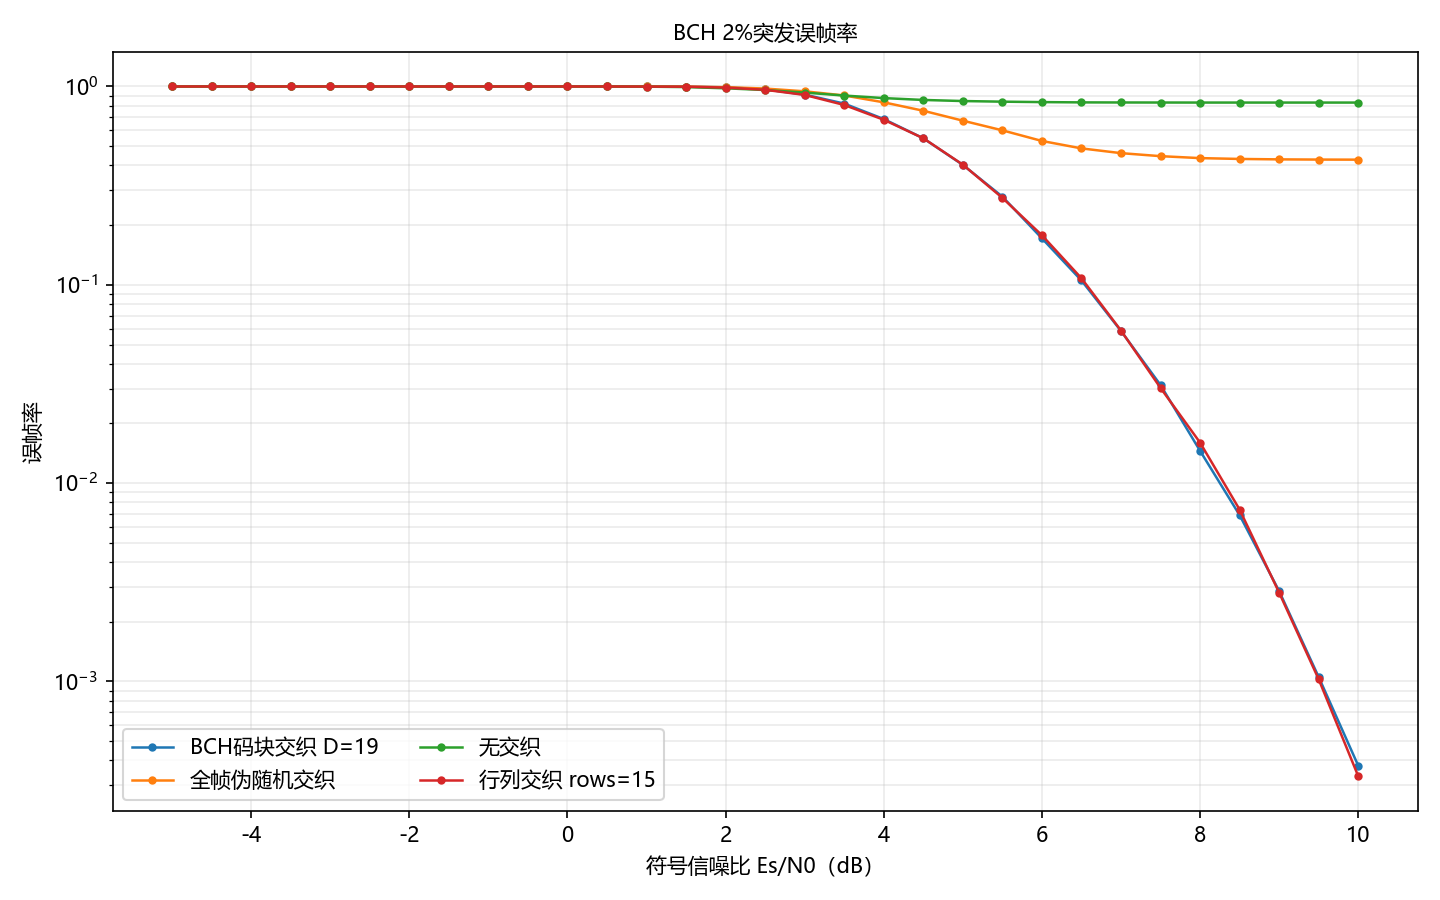
\includegraphics[width=\linewidth]{../Task/Comparison/S7/stage15_scientific_plots/results/bch/03_burst_2_fer/figure.png}\\[-0.2em]
    \small（a）2\%突发
  \end{minipage}
  \hfill
  \begin{minipage}[t]{0.49\textwidth}
    \centering
    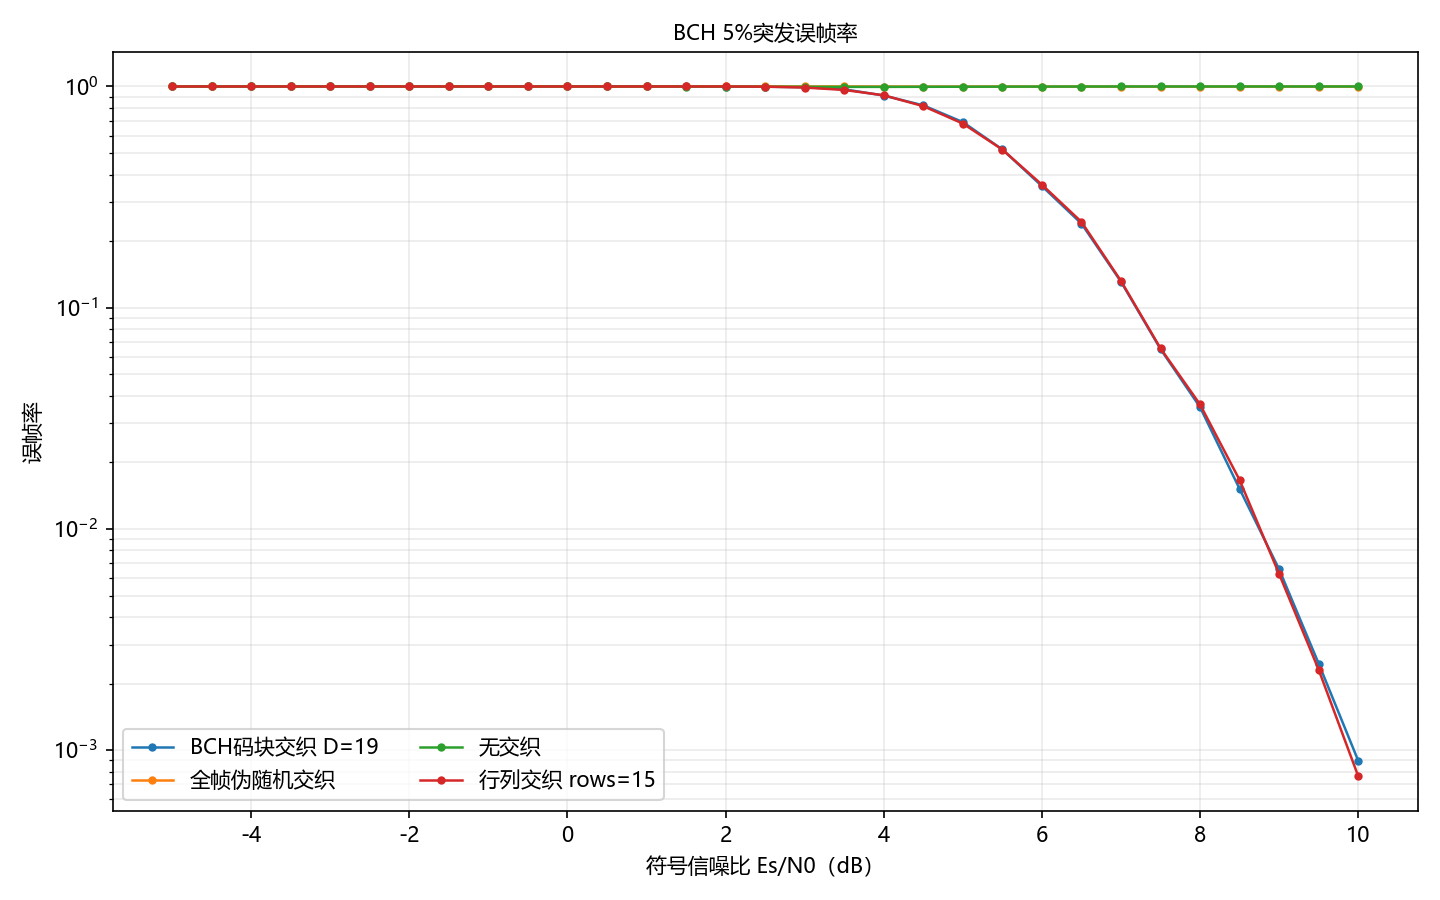
\includegraphics[width=\linewidth]{../Task/Comparison/S7/stage15_scientific_plots/results/bch/04_burst_5_fer/figure.png}\\[-0.2em]
    \small（b）5\%突发
  \end{minipage}
  \caption{分块BCH在两档突发长度下的误帧率}
  \label{fig:s7-bch-burst-fer}
\end{figure}

表\ref{tab:s7-bch-fer-improvement}给出$10$ dB代表点的六位置平均、最坏与最好FER。2\%条件下，无交织平均FER为0.829613，子块结构交织和行列交织分别降至$3.77\times10^{-4}$和$3.33\times10^{-4}$；5\%条件下，无交织FER为1，两种规则交织分别为$8.97\times10^{-4}$和$7.63\times10^{-4}$。对应平均FER相对降低率均超过99.9\%。全帧伪随机交织在2\%时平均FER为0.427587，在5\%时为0.998823，表现出置换结构和突发位置之间的强耦合。

\begin{table}[htbp]
  \centering
  \caption{BCH代表性FER改善（$E_s/N_0=10$ dB）}
  \label{tab:s7-bch-fer-improvement}
  \footnotesize
  \begin{tabular}{clrrrr}
    \toprule
    突发 & 配置 & 平均FER & 最坏FER & 最好FER & 相对降低/\% \\
    \midrule
    2\% & 无交织 & 0.829613 & 1 & $2.0\times10^{-5}$ & 0 \\
    2\% & 子块结构$D=19$ & $3.77\times10^{-4}$ & $4.40\times10^{-4}$ & $3.20\times10^{-4}$ & 99.9546 \\
    2\% & 行列$R=15$ & $3.33\times10^{-4}$ & $5.00\times10^{-4}$ & $1.80\times10^{-4}$ & 99.9598 \\
    2\% & 全帧伪随机 & 0.427587 & 0.99998 & $2.60\times10^{-4}$ & 48.4595 \\
    5\% & 无交织 & 1 & 1 & 1 & 0 \\
    5\% & 子块结构$D=19$ & $8.97\times10^{-4}$ & 0.00102 & $8.20\times10^{-4}$ & 99.9103 \\
    5\% & 行列$R=15$ & $7.63\times10^{-4}$ & $8.80\times10^{-4}$ & $6.20\times10^{-4}$ & 99.9237 \\
    5\% & 全帧伪随机 & 0.998823 & 1 & 0.99296 & 0.1177 \\
    \bottomrule
  \end{tabular}
\end{table}

\subsection{两档突发长度的影响}

从突发长度看，6 bit与14 bit连续异常对无交织BCH均构成强烈压力，但规则结构交织后的结果差异较小。$10$ dB时，子块结构交织由2\%条件的$3.77\times10^{-4}$上升到5\%条件的$8.97\times10^{-4}$，行列交织由$3.33\times10^{-4}$上升到$7.63\times10^{-4}$；两者的最坏位置FER仍不高于0.00102。由于BCH(15,11,1)只能保证纠正每个子块中的单比特错误，14 bit异常能否被有效处理取决于逆置换后每个子块获得的错误数，而不是只取决于总错误数。

全帧伪随机配置呈现不同特征。2\%条件下其最好位置FER已降到$2.60\times10^{-4}$，但最坏位置仍为0.99998，导致六位置平均FER为0.427587；5\%条件下最好位置也达到0.99296。该结果表明，固定伪随机置换可能在部分起点形成有利分散，却没有在所有代表位置上保持一致。规则结构交织把连续输入位置映射到可预期的子块关系，对本章19子块结构形成更稳定的覆盖。因此，评价交织方法时应同时查看平均、最坏和最好位置，而不能从单一有利起点形成整体结论。

\subsection{FER改善与突发错误容限}

以FER不高于0.1作为高工作点判据，子块结构$D=19$和行列$R=15$在两档已测试突发条件下均满足门限。这里的“容限”只表示离散测试网格中的通过状态：已知2\%和5\%两点通过，并不据此估计两点之间或更长突发下的临界比例。无交织和全帧伪随机配置在2\%最坏位置已经不满足门限，说明只报告平均FER会低估位置风险。规则结构交织同时取得较低平均FER和较低最坏位置FER，因而其推荐依据包含性能水平与位置稳定性两部分。

行列$R=15$与子块结构$D=19$的高工作点结果非常接近：5\%条件下前者平均FER低$1.33\times10^{-4}$，后者最坏位置FER高$1.40\times10^{-4}$。这些差值来自相同帧序列和噪声条件下的正式统计，可以用于当前配置排序，但不应放大为普遍性的算法差距。两者缓存量相同，软件交织和去交织时间也处于相近范围；工程选择可进一步结合映射实现便利性和存储访问方式。

5\%条件下的FER绝对改善量和相对降低率见图\ref{fig:s7-bch-fer-gain}。两种规则结构交织的收益主要出现在中高信噪比区；低信噪比区由AWGN与突发共同作用，所有配置的FER均接近1，交织映射难以形成可分辨收益。进入较高信噪比后，AWGN造成的分散错误减少，连续突发的空间结构成为主导因素，规则交织的作用随之显现。

\begin{figure}[htbp]
  \centering
  \begin{minipage}[t]{0.49\textwidth}
    \centering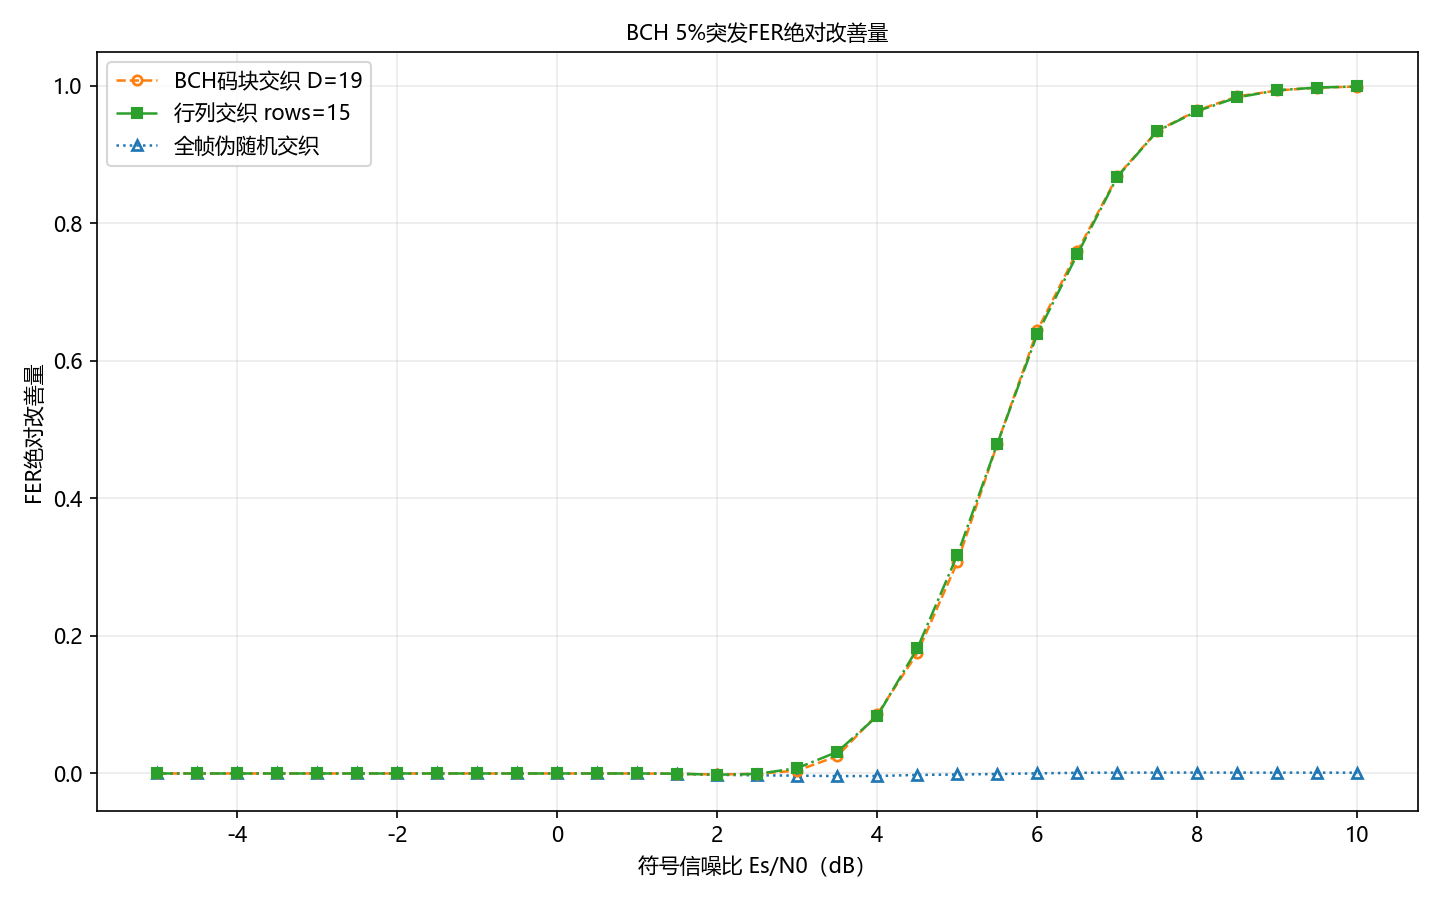
\includegraphics[width=\linewidth]{../Task/Comparison/S7/stage15_scientific_plots/results/bch/11_absoluteFerImprovement/figure.png}\\[-0.2em]
    \small（a）FER绝对改善量
  \end{minipage}\hfill
  \begin{minipage}[t]{0.49\textwidth}
    \centering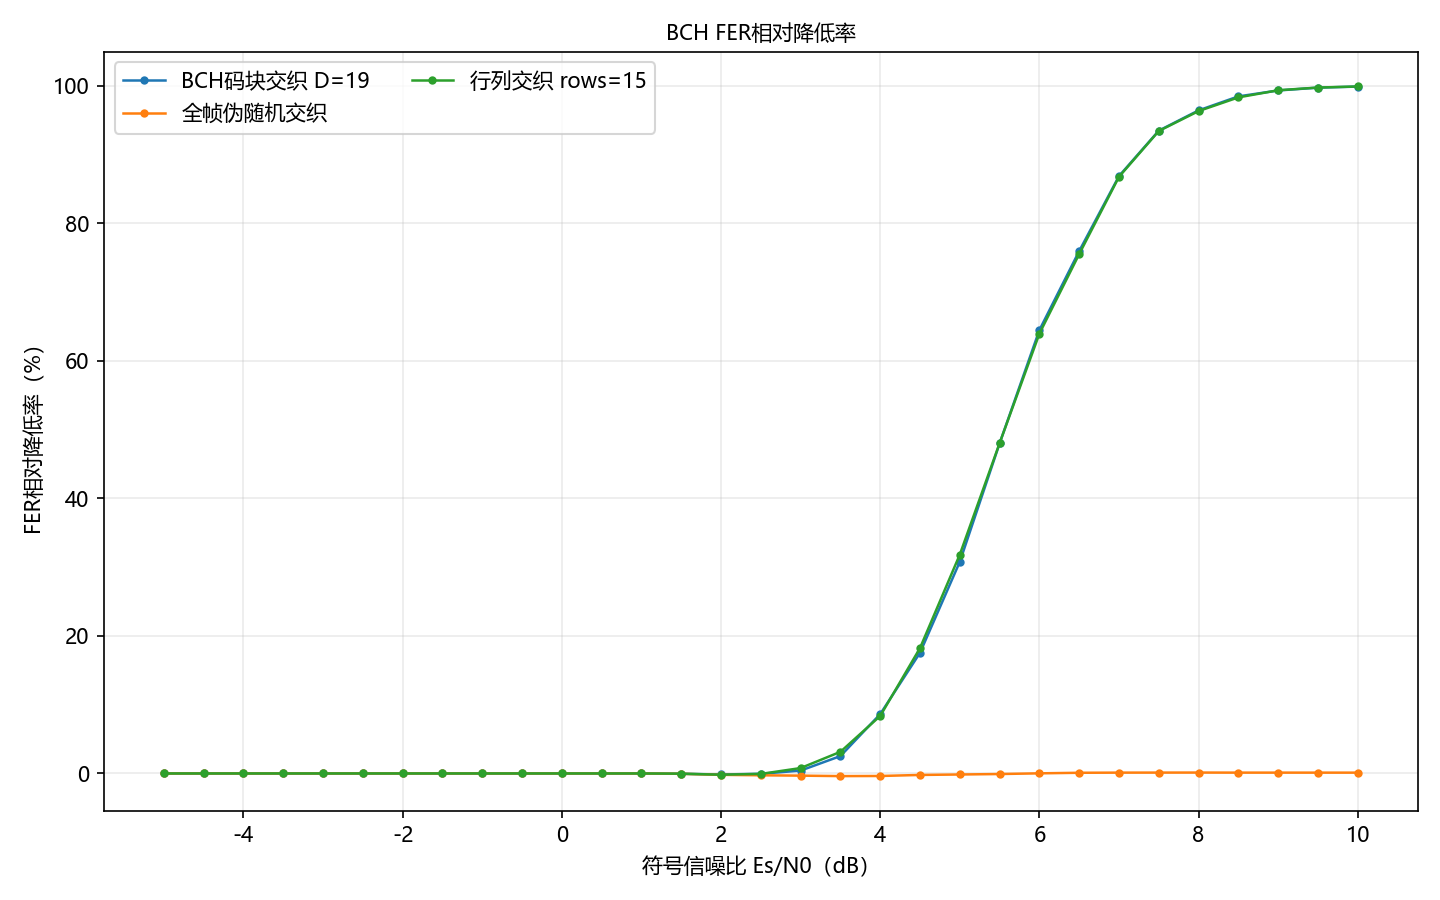
\includegraphics[width=\linewidth]{../Task/Comparison/S7/stage15_scientific_plots/results/bch/12_relativeFerReductionPercent/figure.png}\\[-0.2em]
    \small（b）FER相对降低率
  \end{minipage}
  \caption{5\%突发条件下BCH交织的FER改善}
  \label{fig:s7-bch-fer-gain}
\end{figure}

\subsection{突发位置敏感性}

图\ref{fig:s7-bch-position-statistics}给出六位置平均、最坏和最好FER，图\ref{fig:s7-bch-position-detail}进一步给出推荐行列配置的六条位置曲线与各配置的位置敏感度。无交织和全帧伪随机配置在最好与最坏位置之间存在较大差异；子块结构交织与行列交织在高信噪比区的三类统计量更接近，表明规则映射降低了特定突发起点与子块边界重合所造成的波动。

\begin{figure}[htbp]
  \centering
  \begin{minipage}[t]{0.32\textwidth}
    \centering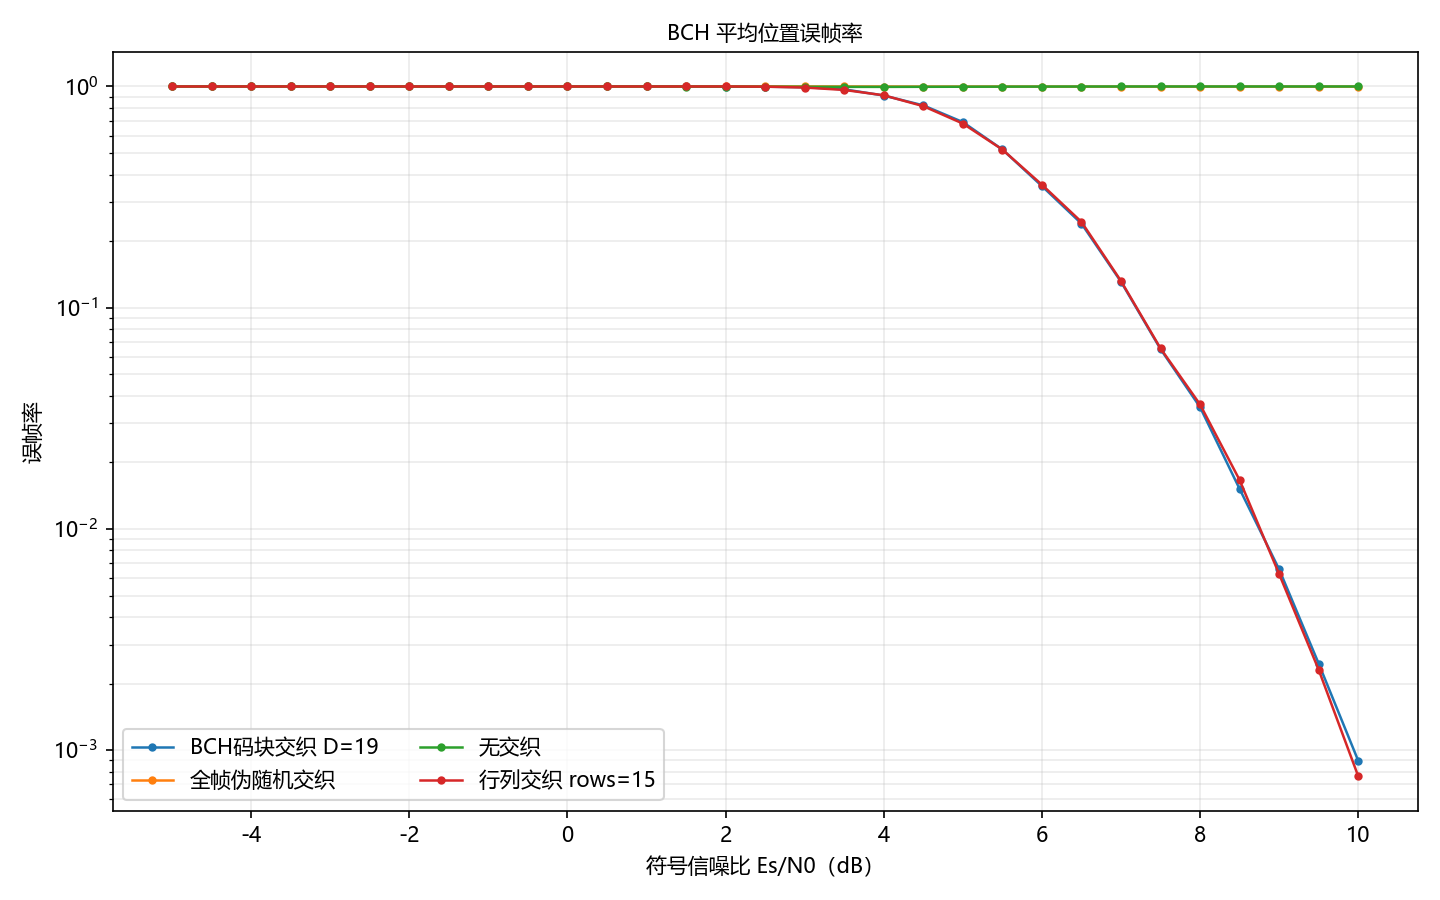
\includegraphics[width=\linewidth]{../Task/Comparison/S7/stage15_scientific_plots/results/bch/07_mean_position_fer/figure.png}\\[-0.2em]\small（a）六位置平均
  \end{minipage}\hfill
  \begin{minipage}[t]{0.32\textwidth}
    \centering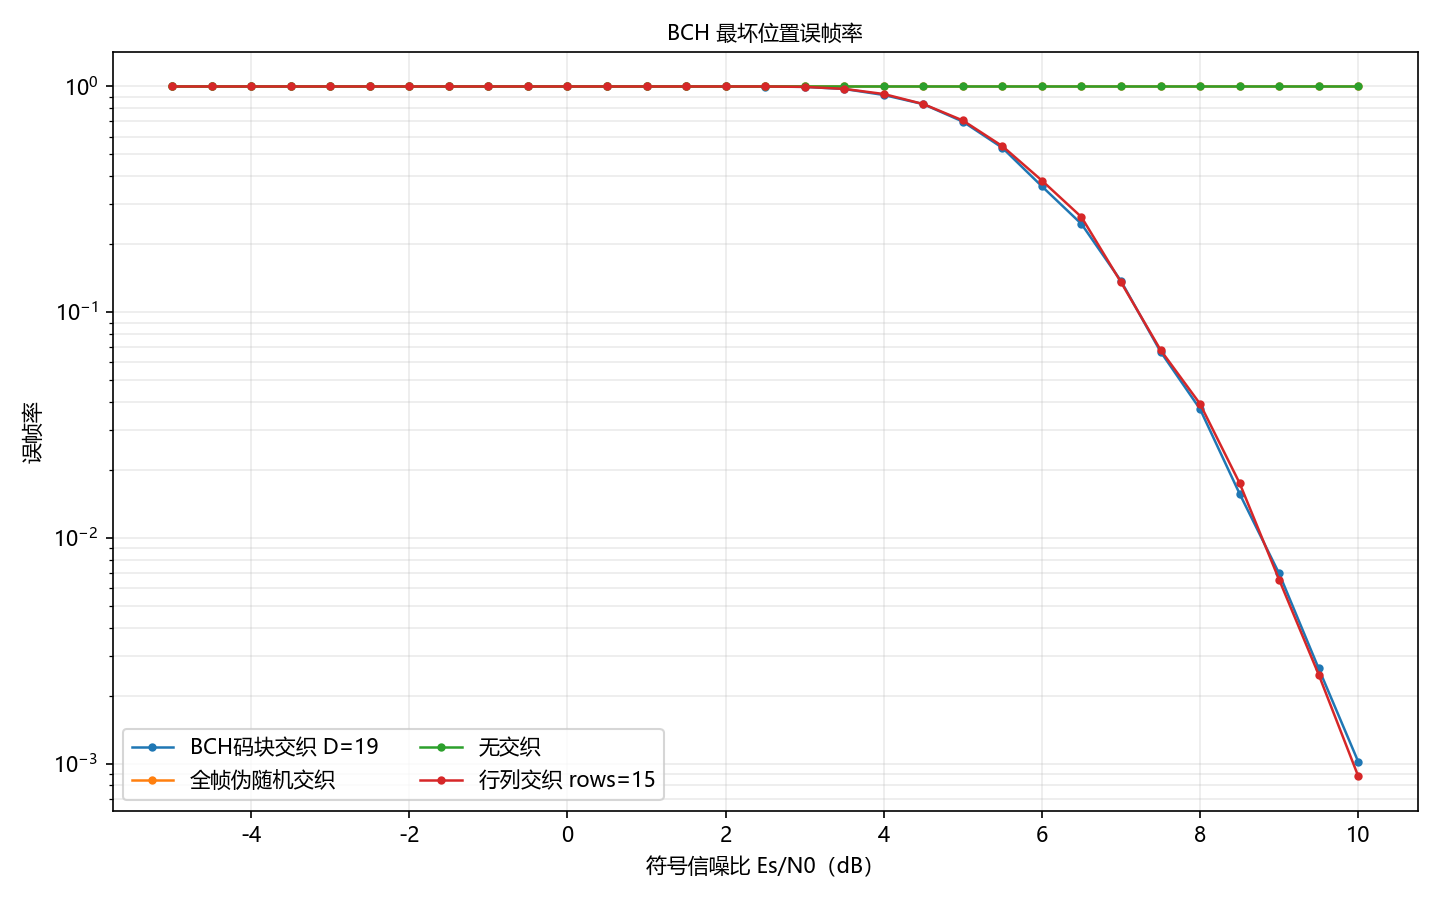
\includegraphics[width=\linewidth]{../Task/Comparison/S7/stage15_scientific_plots/results/bch/08_max_position_fer/figure.png}\\[-0.2em]\small（b）最坏位置
  \end{minipage}\hfill
  \begin{minipage}[t]{0.32\textwidth}
    \centering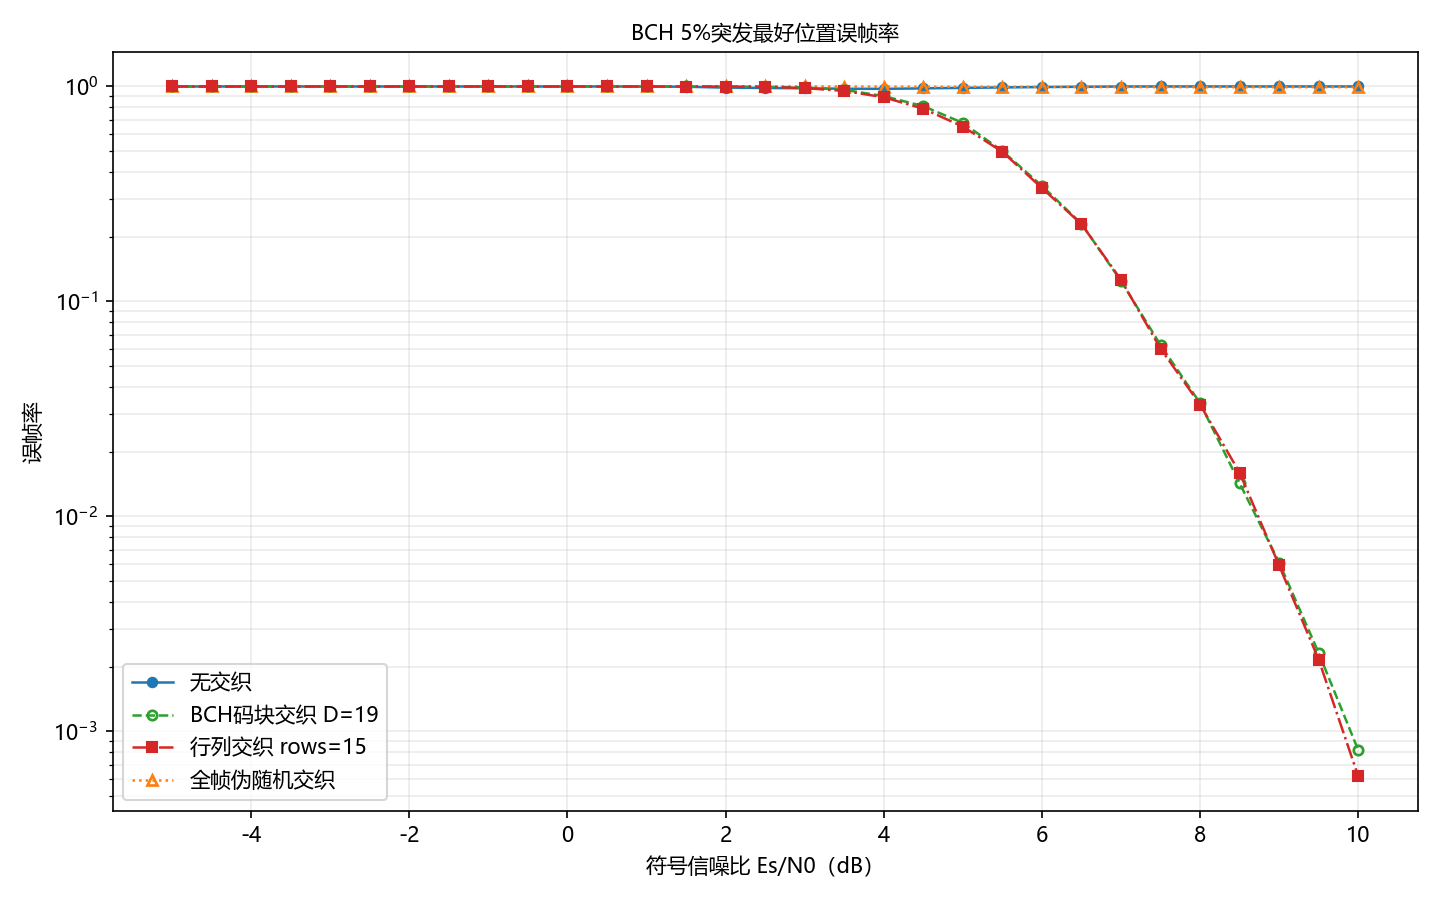
\includegraphics[width=\linewidth]{../Task/Comparison/S7/stage15_scientific_plots/results/bch/09_min_position_fer/figure.png}\\[-0.2em]\small（c）最好位置
  \end{minipage}
  \caption{5\%突发条件下BCH位置统计结果}
  \label{fig:s7-bch-position-statistics}
\end{figure}

\begin{figure}[htbp]
  \centering
  \begin{minipage}[t]{0.49\textwidth}
    \centering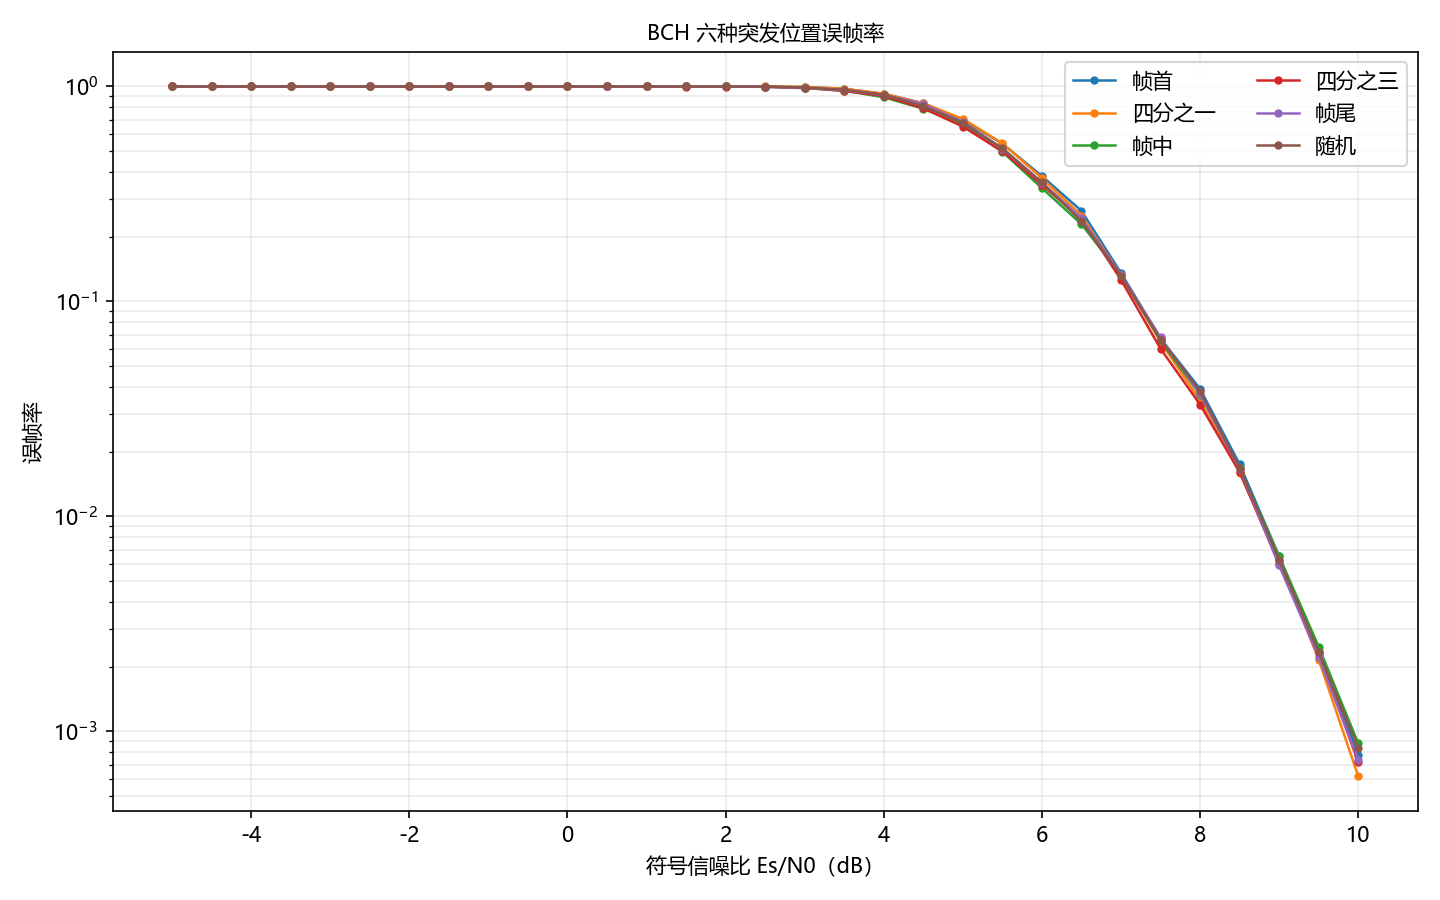
\includegraphics[width=\linewidth]{../Task/Comparison/S7/stage15_scientific_plots/results/bch/06_six_positions_fer/figure.png}\\[-0.2em]\small（a）推荐配置的六位置FER
  \end{minipage}\hfill
  \begin{minipage}[t]{0.49\textwidth}
    \centering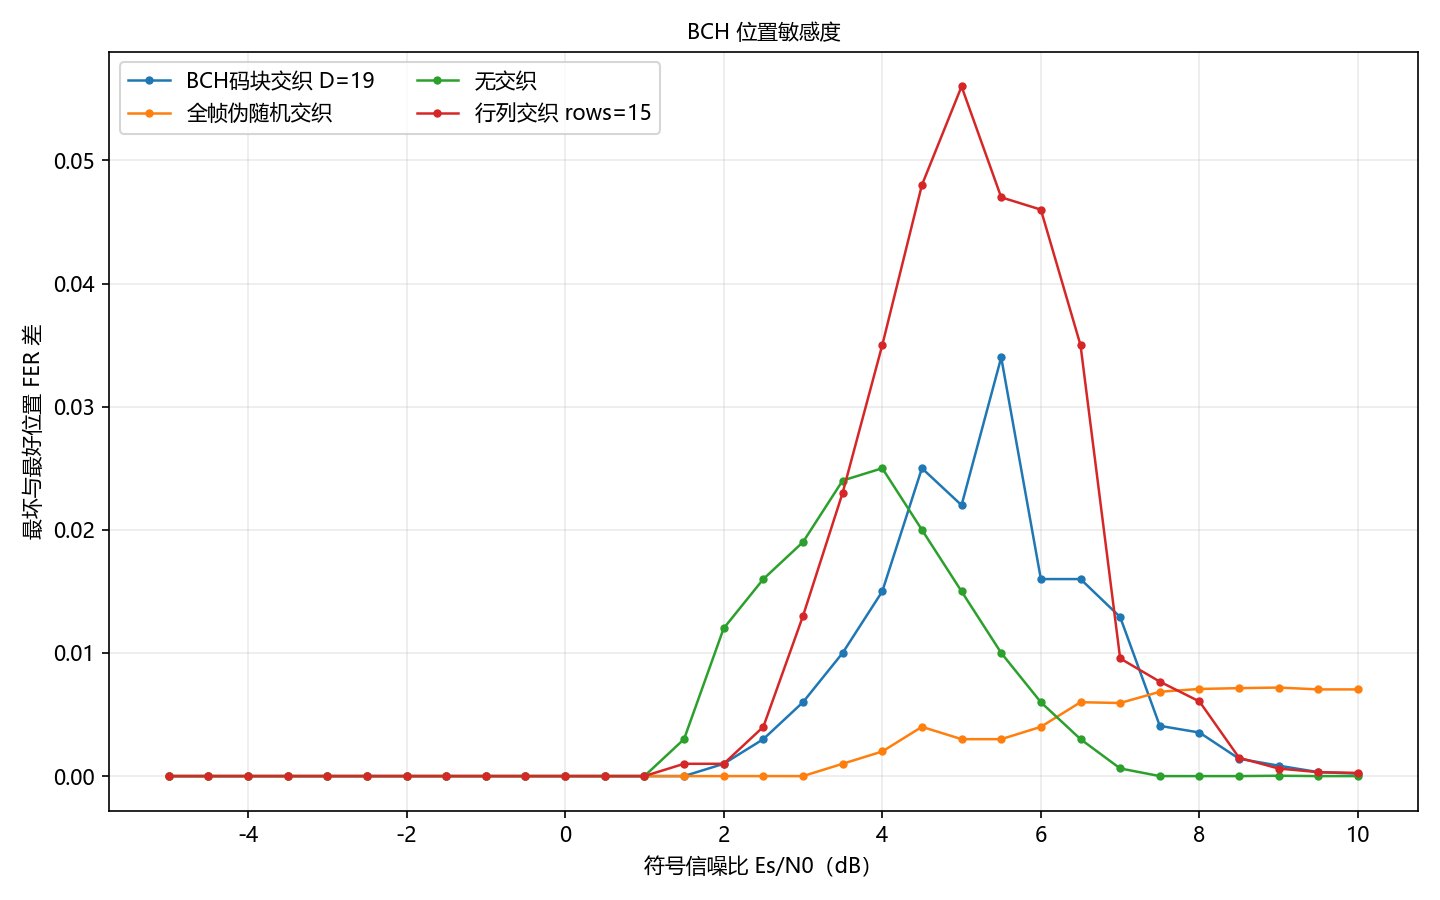
\includegraphics[width=\linewidth]{../Task/Comparison/S7/stage15_scientific_plots/results/bch/10_position_sensitivity/figure.png}\\[-0.2em]\small（b）最坏与最好位置FER差
  \end{minipage}
  \caption{5\%突发条件下BCH突发位置敏感性}
  \label{fig:s7-bch-position-detail}
\end{figure}

全起点扫描为六位置结果提供了更细粒度的验证。图\ref{fig:s7-bch-heatmaps}中，2\%与5\%热力图均保留每个已测试起点的原始FER，不对未测试位置插值。2\%条件下不同起点的差异更容易分辨；5\%条件下，规则结构交织仍保持较低的高工作点FER，而无交织与全帧伪随机配置在多数起点上维持高错误率。该结果说明六个代表位置没有掩盖主要的结构性差异。

\begin{figure}[htbp]
  \centering
  \begin{minipage}[t]{0.49\textwidth}
    \centering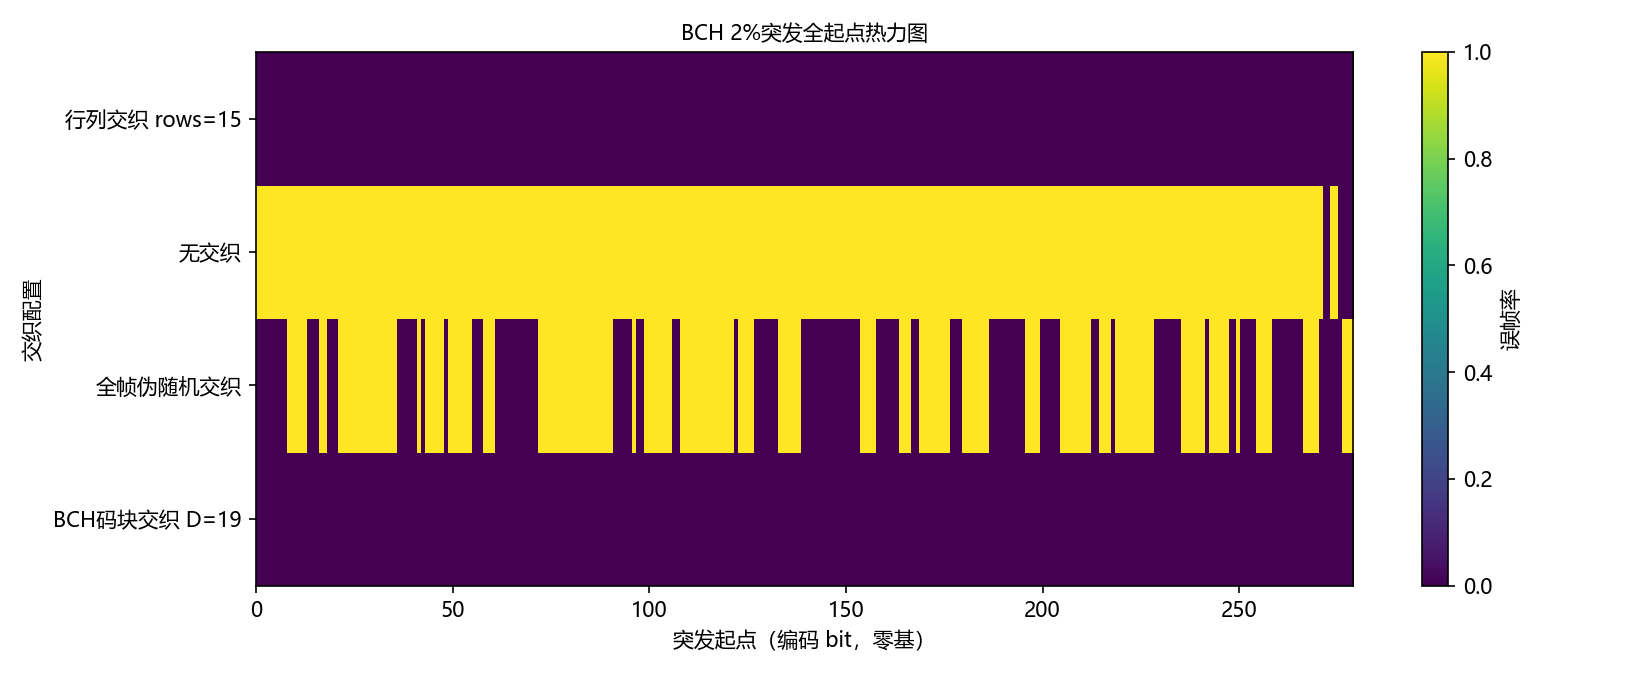
\includegraphics[width=\linewidth]{../Task/Comparison/S7/stage15_scientific_plots/results/bch/21_all_start_heatmap_2_percent/figure.png}\\[-0.2em]\small（a）2\%突发
  \end{minipage}\hfill
  \begin{minipage}[t]{0.49\textwidth}
    \centering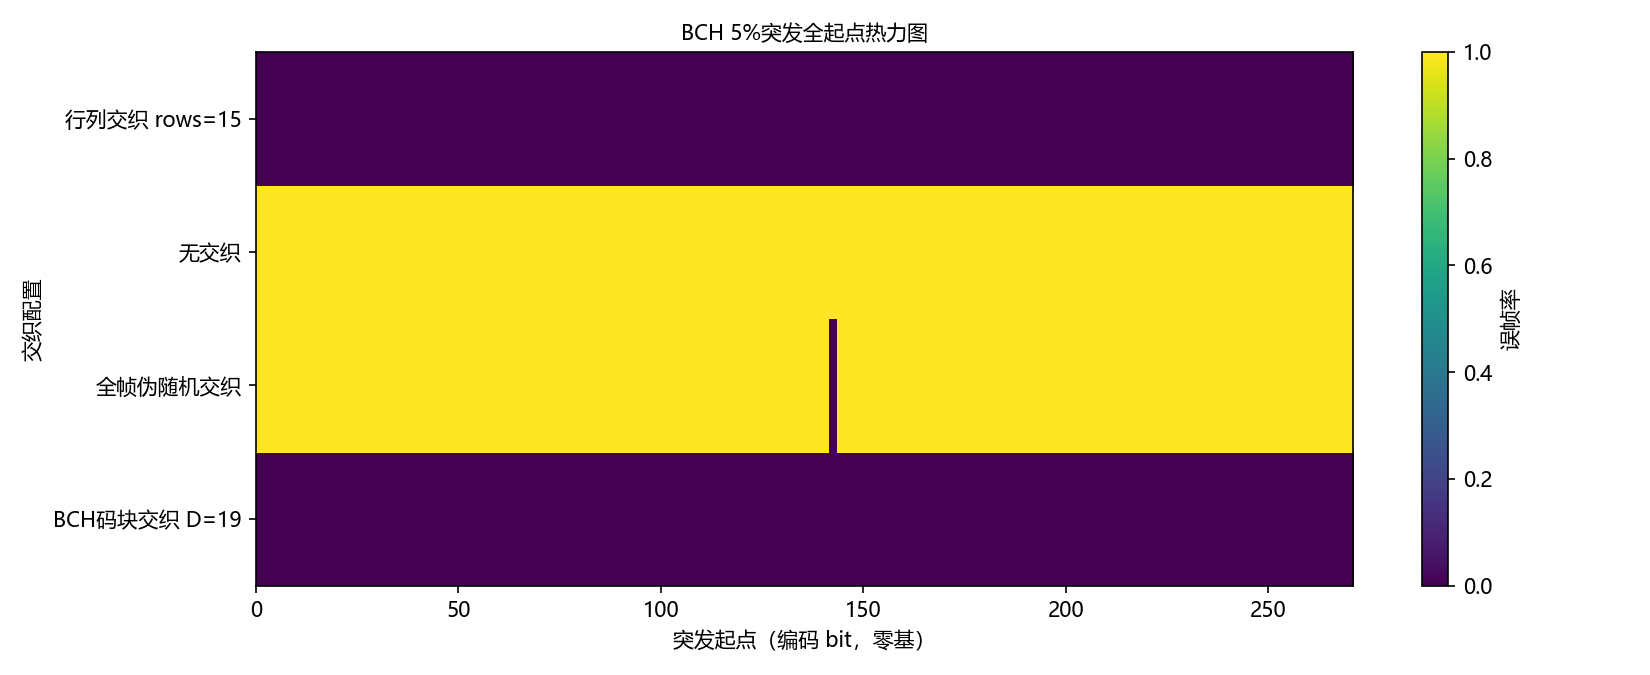
\includegraphics[width=\linewidth]{../Task/Comparison/S7/stage15_scientific_plots/results/bch/22_all_start_heatmap_5_percent/figure.png}\\[-0.2em]\small（b）5\%突发
  \end{minipage}
  \caption{BCH高工作点全起点FER热力图}
  \label{fig:s7-bch-heatmaps}
\end{figure}

\subsection{错误跨BCH子块分散机制}

分块BCH的机理可以由受影响子块数与单块最大错误数共同解释。无交织时，连续突发集中落入少量15 bit子块，局部子块可能同时包含多个错误，超过BCH(15,11,1)的单比特保证纠错范围。交织后，同一连续异常经逆置换分散到更多子块，使单个子块内的最大错误数下降，更多子块处于原有单比特可纠正范围。交织没有改变BCH码本或理论纠错能力，而是改善了原有局部纠错能力的利用方式。

图\ref{fig:s7-bch-mechanism}给出行列交织在5\%条件下的两项诊断量。$E_s/N_0=10$ dB时，14 bit突发平均影响约14.0003个子块，单块最大错误数为2。表\ref{tab:s7-bch-mechanism}进一步与其他配置对照：无交织平均只涉及1.4778个子块，但单块最大错误数达到15；全帧伪随机交织涉及约10.7210个子块，单块最大错误数为4；两种规则结构交织均把错误扩展到约14个子块，并把最大值压低至2。该分布变化与表\ref{tab:s7-bch-fer-improvement}中的FER差异一致。

\begin{figure}[htbp]
  \centering
  \begin{minipage}[t]{0.49\textwidth}
    \centering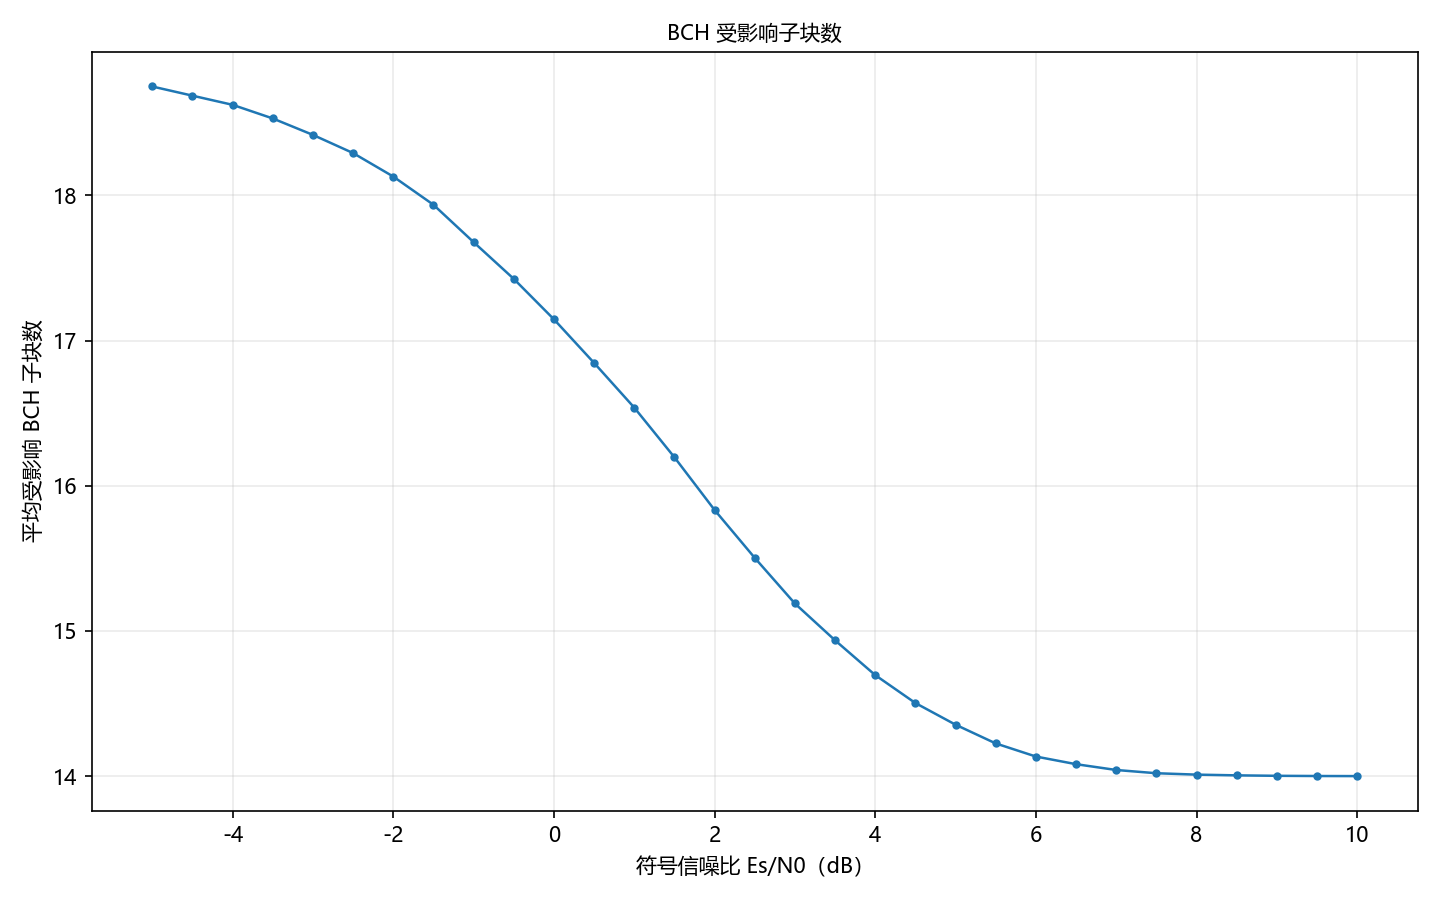
\includegraphics[width=\linewidth]{../Task/Comparison/S7/stage15_scientific_plots/results/bch/14_affected_bch_blocks/figure.png}\\[-0.2em]\small（a）平均受影响子块数
  \end{minipage}\hfill
  \begin{minipage}[t]{0.49\textwidth}
    \centering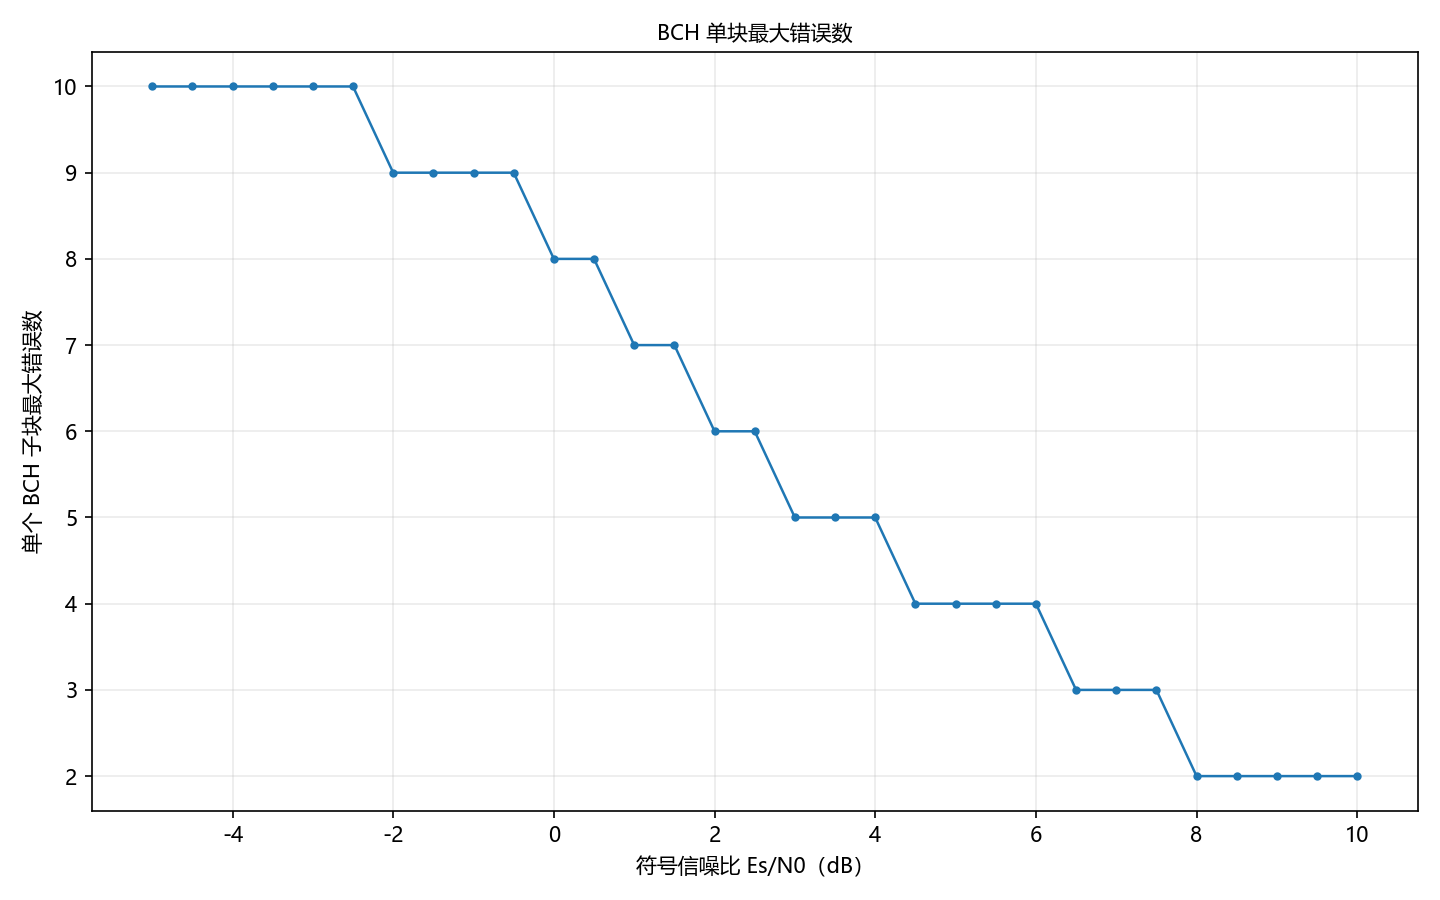
\includegraphics[width=\linewidth]{../Task/Comparison/S7/stage15_scientific_plots/results/bch/15_max_errors_per_block/figure.png}\\[-0.2em]\small（b）单块最大错误数
  \end{minipage}
  \caption{5\%突发条件下BCH错误分散机理证据}
  \label{fig:s7-bch-mechanism}
\end{figure}

\begin{table}[htbp]
  \centering
  \caption{BCH错误分散机制（$E_s/N_0=10$ dB，5\%突发）}
  \label{tab:s7-bch-mechanism}
  \small
  \begin{tabular}{lrrrr}
    \toprule
    配置 & 受影响子块均值 & 单块最大错误数 & 纠正子块均值 & 平均FER \\
    \midrule
    无交织 & 1.4778 & 15 & 0.5222 & 1 \\
    子块结构$D=19$ & 14.0003 & 2 & 14.0003 & $8.97\times10^{-4}$ \\
    行列$R=15$ & 14.0003 & 2 & 14.0003 & $7.63\times10^{-4}$ \\
    全帧伪随机 & 10.7210 & 4 & 8.9673 & 0.998823 \\
    \bottomrule
  \end{tabular}
\end{table}

\subsection{缓冲需求与软件处理时间}

三种BCH交织配置均需285 bit结构缓存，见图\ref{fig:s7-bch-buffer}。仅按2\%和5\%正式仿真数据进行帧数加权后，无交织、子块结构、行列和全帧伪随机配置的软件交织CPU时间分别为328.4、324.9、325.3和325.1 ns/帧；去交织时间分别为310.5、329.9、322.6和324.6 ns/帧。交织函数本身的时间差小于十纳秒量级，译码CPU时间约为$8.42\sim9.00~\mu$s/帧。上述数值是\texttt{steady\_clock}包围软件函数得到的处理时间，不包括编码、调制、信道，也不能直接换算为硬件时延。

\begin{figure}[htbp]
  \centering
  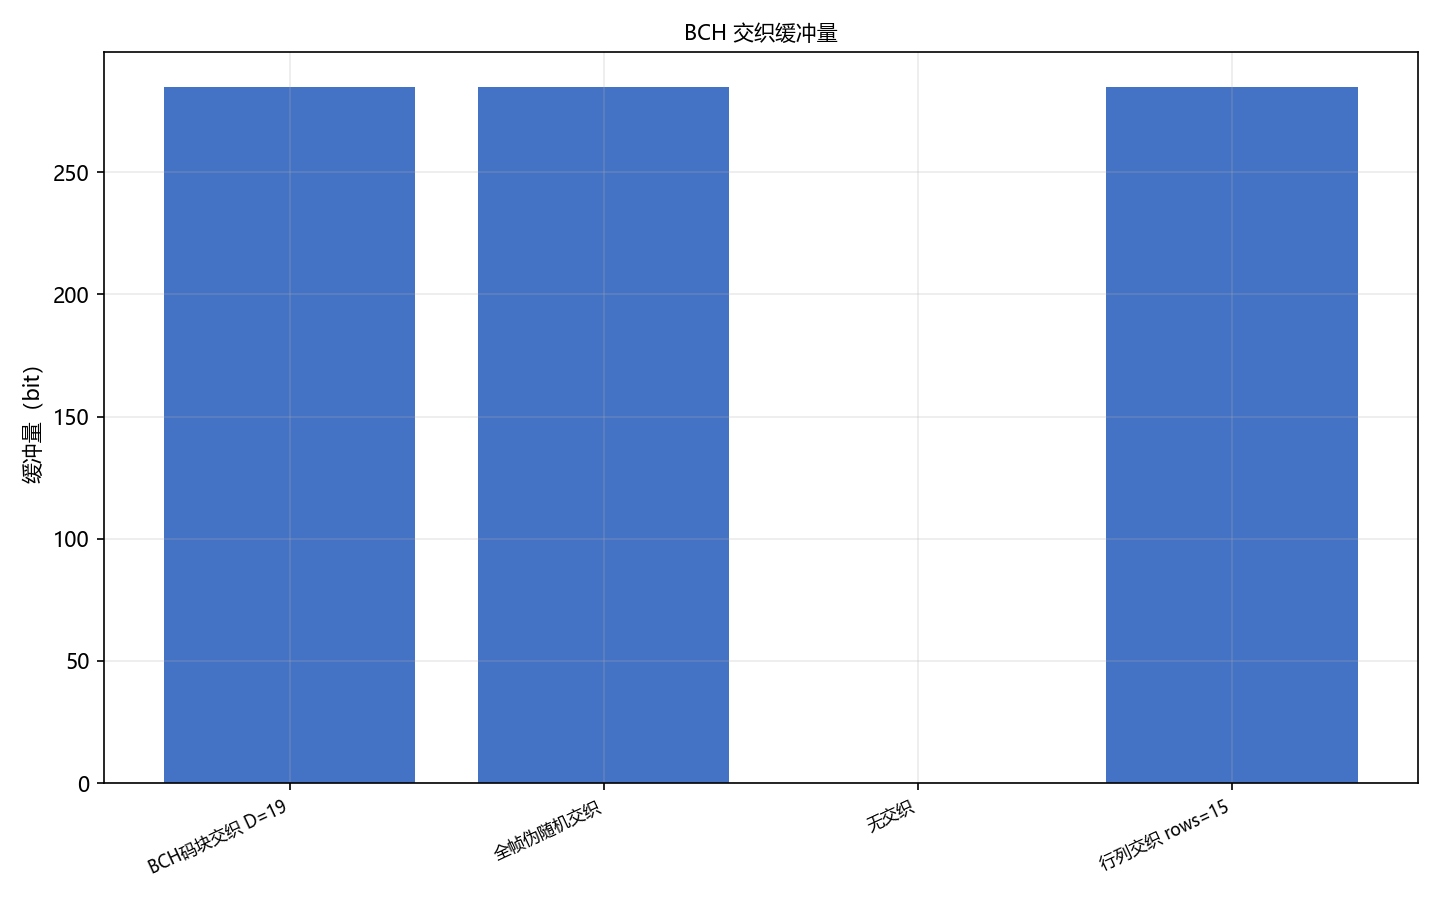
\includegraphics[width=0.88\textwidth]{../Task/Comparison/S7/stage15_scientific_plots/results/bch/19_bufferBits/figure.png}
  \caption{BCH交织配置的结构缓存量}
  \label{fig:s7-bch-buffer}
\end{figure}

\section{卷积码交织抗突发错误结果}

\subsection{不同交织配置总体BER与FER}

图\ref{fig:s7-cc-burst-fer}给出2\%和5\%突发下卷积码FER。图中的LDPC曲线是无交织、无突发AWGN近码率基线，只用于高速编码方案参考，不表示LDPC经历对应的突发错误条件。2\%条件下，局部伪随机Pseudo128和短深度$D=8$在高信噪比区降低了平均FER；5\%条件下，各卷积码配置在当前$E_s/N_0$上限附近仍接近FER饱和区，因而不能从本测试范围给出稳定的低FER工作点。

\begin{figure}[htbp]
  \centering
  \begin{minipage}[t]{0.49\textwidth}
    \centering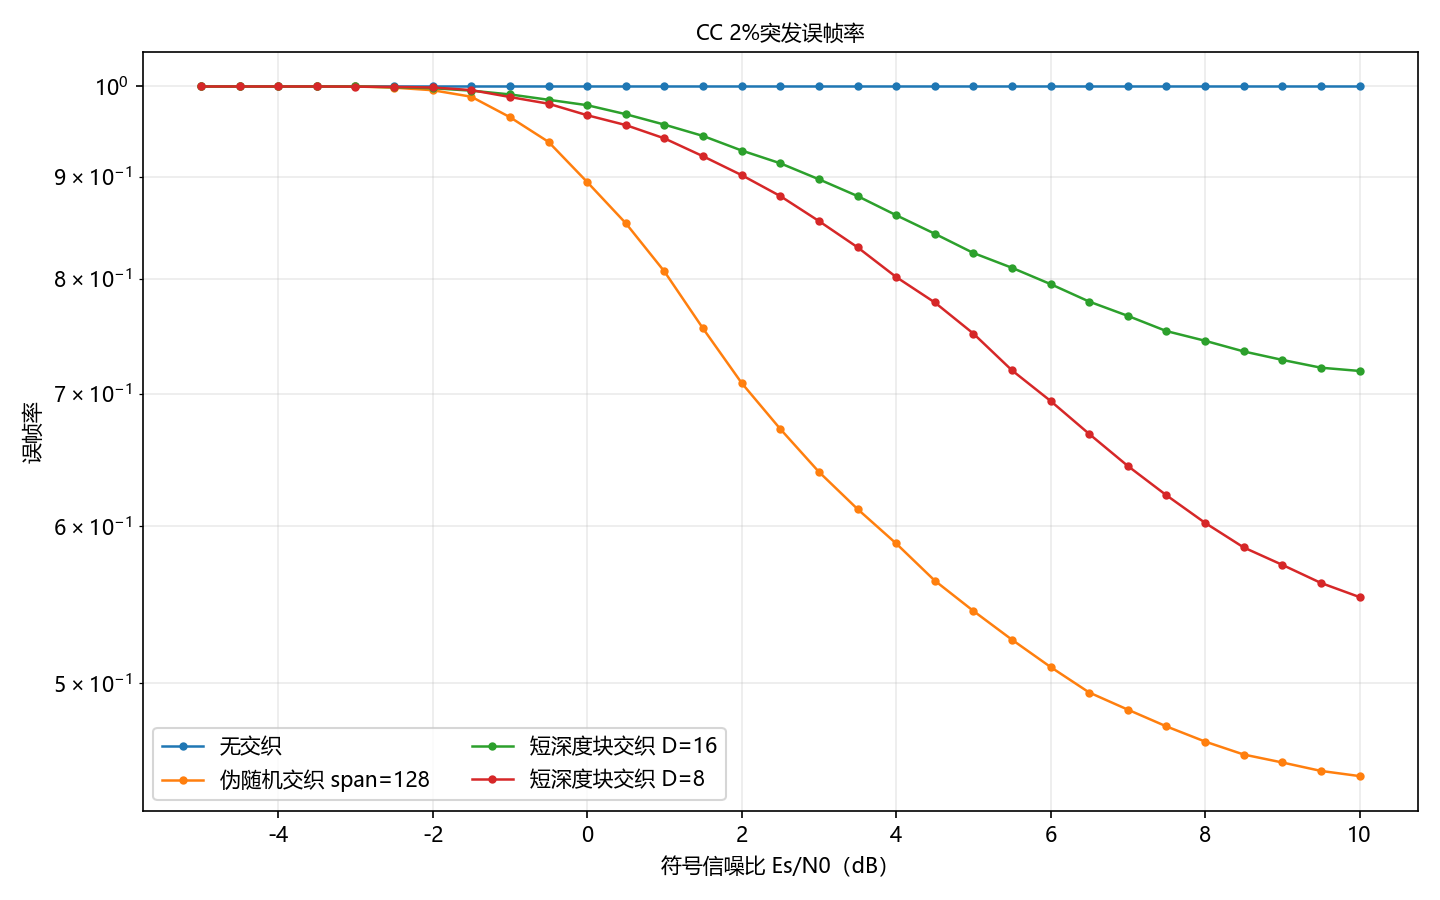
\includegraphics[width=\linewidth]{../Task/Comparison/S7/stage15_scientific_plots/results/cc/03_burst_2_fer/figure.png}\\[-0.2em]\small（a）2\%突发
  \end{minipage}\hfill
  \begin{minipage}[t]{0.49\textwidth}
    \centering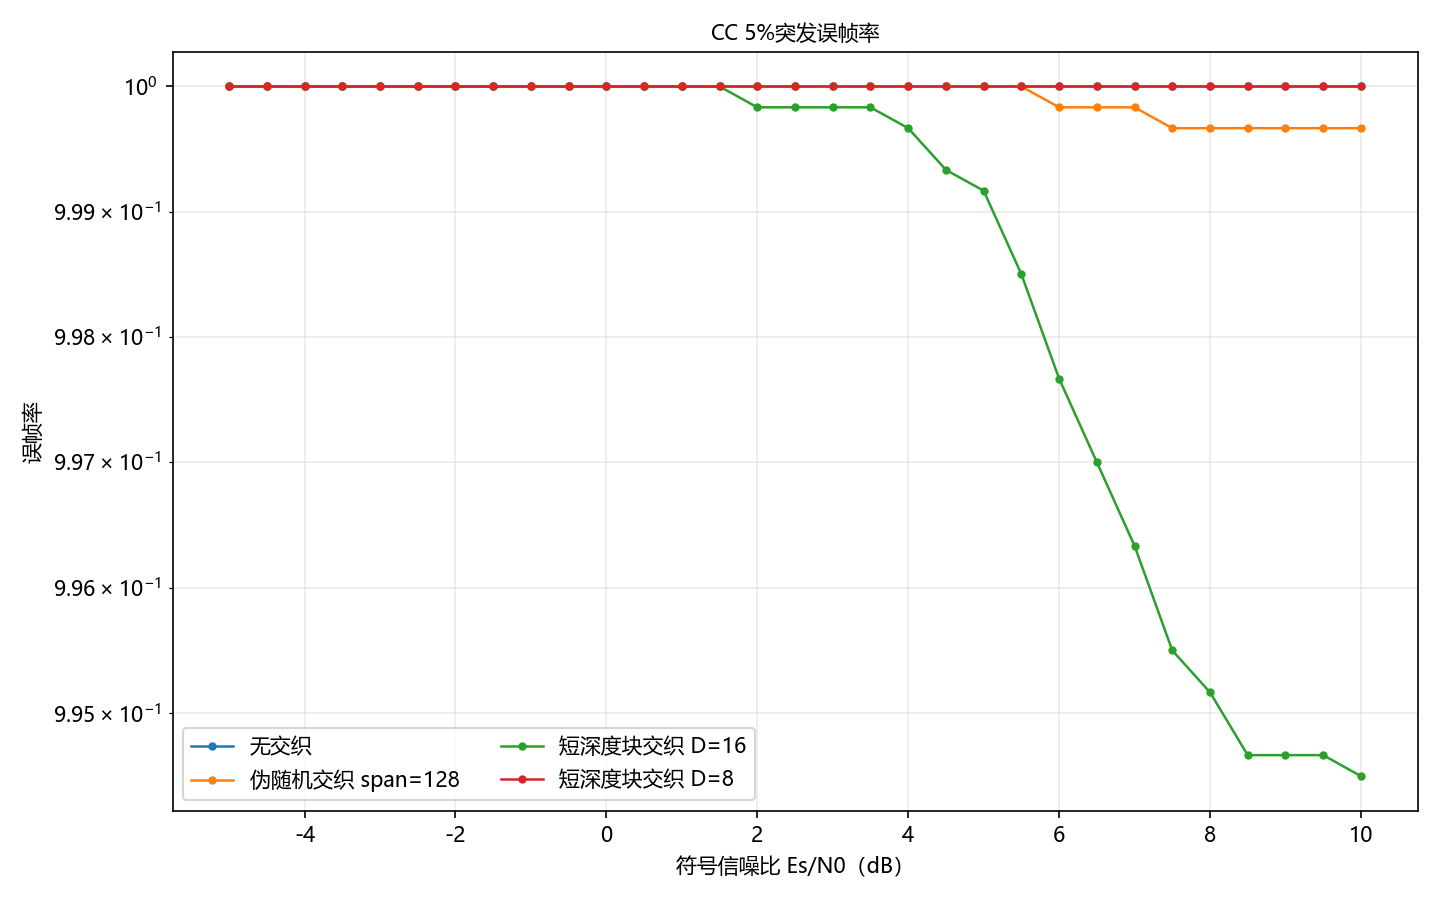
\includegraphics[width=\linewidth]{../Task/Comparison/S7/stage15_scientific_plots/results/cc/04_burst_5_fer/figure.png}\\[-0.2em]\small（b）5\%突发
  \end{minipage}
  \caption{卷积码在两档突发长度下的误帧率。LDPC曲线为无突发AWGN近码率基线，不表示LDPC经历突发错误}
  \label{fig:s7-cc-burst-fer}
\end{figure}

表\ref{tab:s7-cc-fer-improvement}给出$10$ dB定量结果。2\%条件下，无交织FER为1，$D=8$、Pseudo128和$D=16$的六位置平均FER分别为0.552654、0.448905和0.718629，相对无交织分别下降44.73\%、55.11\%和28.14\%。5\%条件下，三种交织配置的平均FER均不低于0.9945，最坏位置FER均为1。该结果支持交织对较短突发具有可观测收益，同时也限定了本卷积码配置在31 bit连续异常下的能力边界。

\begin{table}[htbp]
  \centering
  \caption{卷积码代表性FER改善（$E_s/N_0=10$ dB）}
  \label{tab:s7-cc-fer-improvement}
  \footnotesize
  \begin{tabular}{clrrrr}
    \toprule
    突发 & 配置 & 平均FER & 最坏FER & 最好FER & 相对降低/\% \\
    \midrule
    2\% & 无交织 & 1 & 1 & 1 & 0 \\
    2\% & 短深度$D=8$ & 0.552654 & 0.85 & 0.063805 & 44.7346 \\
    2\% & Pseudo128 & 0.448905 & 0.84 & 0.004165 & 55.1095 \\
    2\% & 短深度$D=16$ & 0.718629 & 1 & 0.498 & 28.1371 \\
    5\% & 无交织 & 1 & 1 & 1 & 0 \\
    5\% & 短深度$D=8$ & 1 & 1 & 1 & 0 \\
    5\% & Pseudo128 & 0.999667 & 1 & 0.998 & 0.0333 \\
    5\% & 短深度$D=16$ & 0.994500 & 1 & 0.984 & 0.5500 \\
    \bottomrule
  \end{tabular}
\end{table}

\subsection{两档突发长度的影响}

12 bit突发与31 bit突发呈现出不同的可恢复区间。2\%条件下，Pseudo128和$D=8$在$10$ dB处分别把平均FER降至0.448905和0.552654，最好位置FER分别达到0.004165和0.063805，说明较短连续异常经逆置换后能够减少对相邻路径度量的集中作用。然而两者最坏位置FER仍为0.84和0.85，位置依赖没有消失。$D=16$在相同工作点的平均FER为0.718629，表明更大规则块深度并不自动带来更低FER。

31 bit突发覆盖约15.5个母码输出对。在当前最高$E_s/N_0$下，$D=8$平均FER仍为1，Pseudo128和$D=16$分别为0.999667和0.994500，且所有配置最坏位置FER均为1。AWGN继续降低时，突发造成的连续异常仍足以维持路径竞争错误，形成高FER平台。该数据边界意味着卷积码交织的工程建议主要由2\%条件支撑；5\%结果用于界定当前配置的不足，不能用极小的平均差值声称已经形成稳定改善。

FER与BER反映的侧面并不完全相同。图\ref{fig:s7-cc-ber}显示5\%条件下各配置的BER曲线；在$10$ dB时，无交织、$D=8$、Pseudo128和$D=16$的平均BER分别为0.016864、0.089080、0.069413和0.129994。此时交织后的FER仍接近1，且BER没有相对无交织改善，因此不能只依据局部路径分散机理推断所有误码指标都会同步下降。正式结论以实测FER与BER分别表述。

\begin{figure}[htbp]
  \centering
  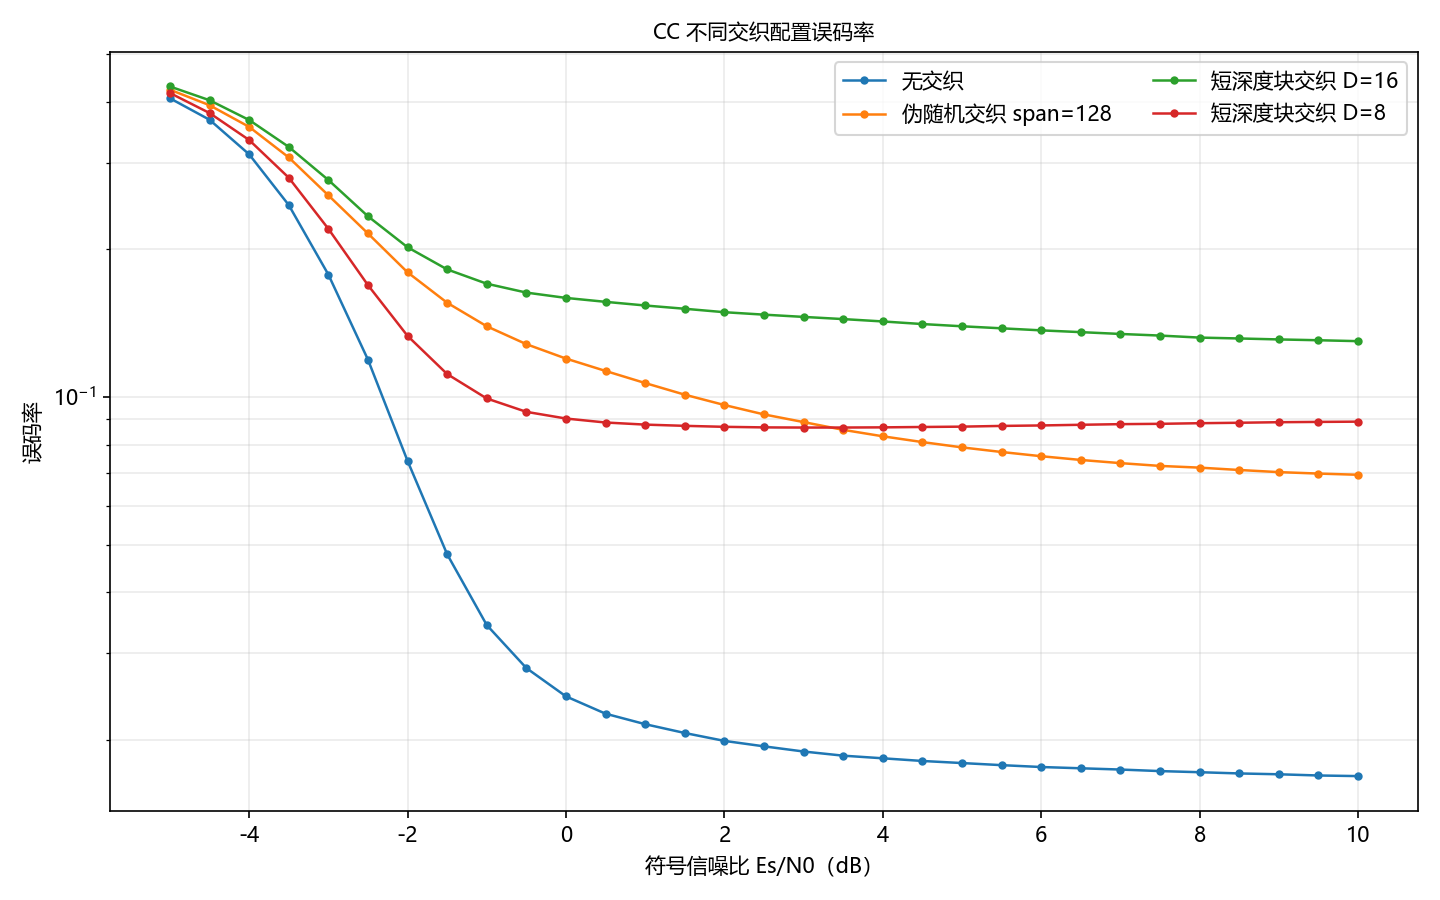
\includegraphics[width=0.88\textwidth]{../Task/Comparison/S7/stage15_scientific_plots/results/cc/02_methods_ber/figure.png}
  \caption{5\%突发条件下卷积码不同交织配置的误码率。LDPC曲线为无突发AWGN近码率基线}
  \label{fig:s7-cc-ber}
\end{figure}

\subsection{突发位置敏感性}

图\ref{fig:s7-cc-position-statistics}给出5\%条件下的平均、最坏和最好位置FER。由于多数曲线处于FER饱和区，三类统计量的间距有限；图\ref{fig:s7-cc-position-detail}中的六位置曲线和敏感度仍表明，2\%较短突发下不同起点会显著改变局部路径竞争，尤其在高信噪比区更易形成可见差异。位置敏感性必须与突发比例和工作点联合解释，不能只用单一最坏位置替代完整统计。

\begin{figure}[htbp]
  \centering
  \begin{minipage}[t]{0.32\textwidth}
    \centering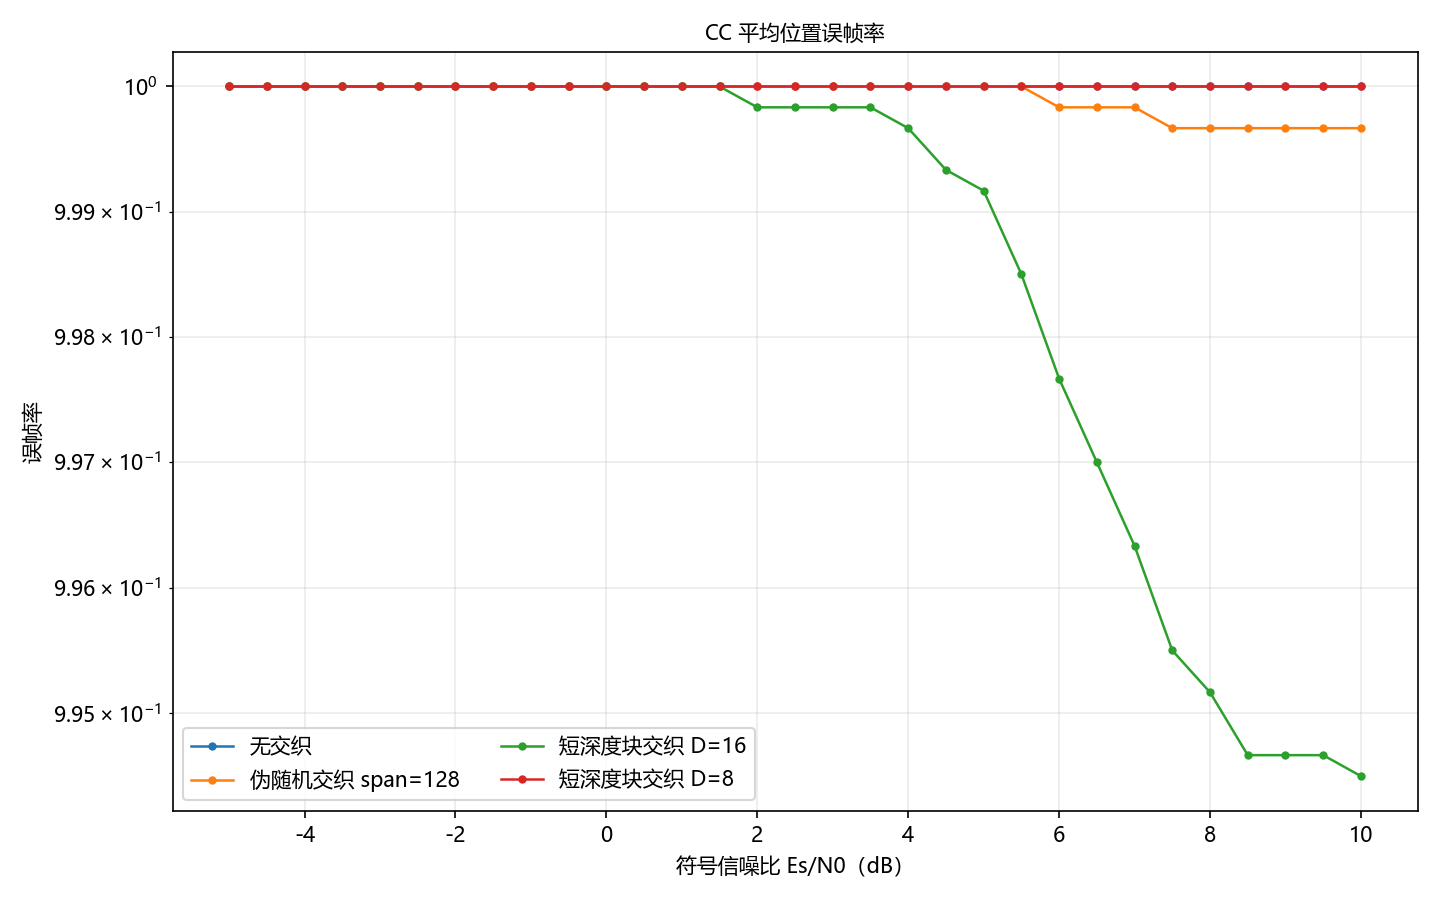
\includegraphics[width=\linewidth]{../Task/Comparison/S7/stage15_scientific_plots/results/cc/07_mean_position_fer/figure.png}\\[-0.2em]\small（a）六位置平均
  \end{minipage}\hfill
  \begin{minipage}[t]{0.32\textwidth}
    \centering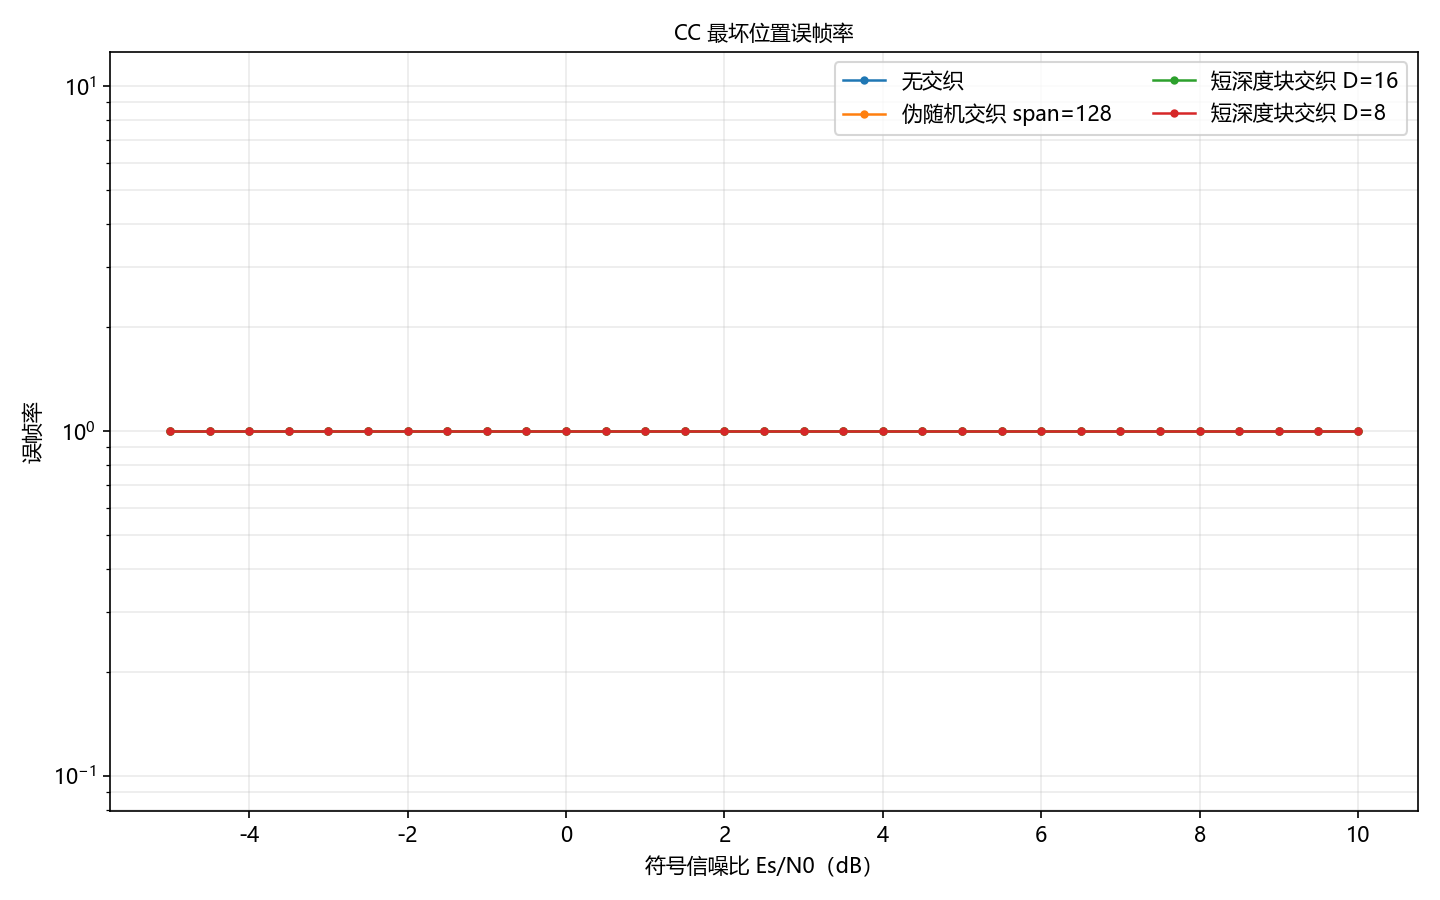
\includegraphics[width=\linewidth]{../Task/Comparison/S7/stage15_scientific_plots/results/cc/08_max_position_fer/figure.png}\\[-0.2em]\small（b）最坏位置
  \end{minipage}\hfill
  \begin{minipage}[t]{0.32\textwidth}
    \centering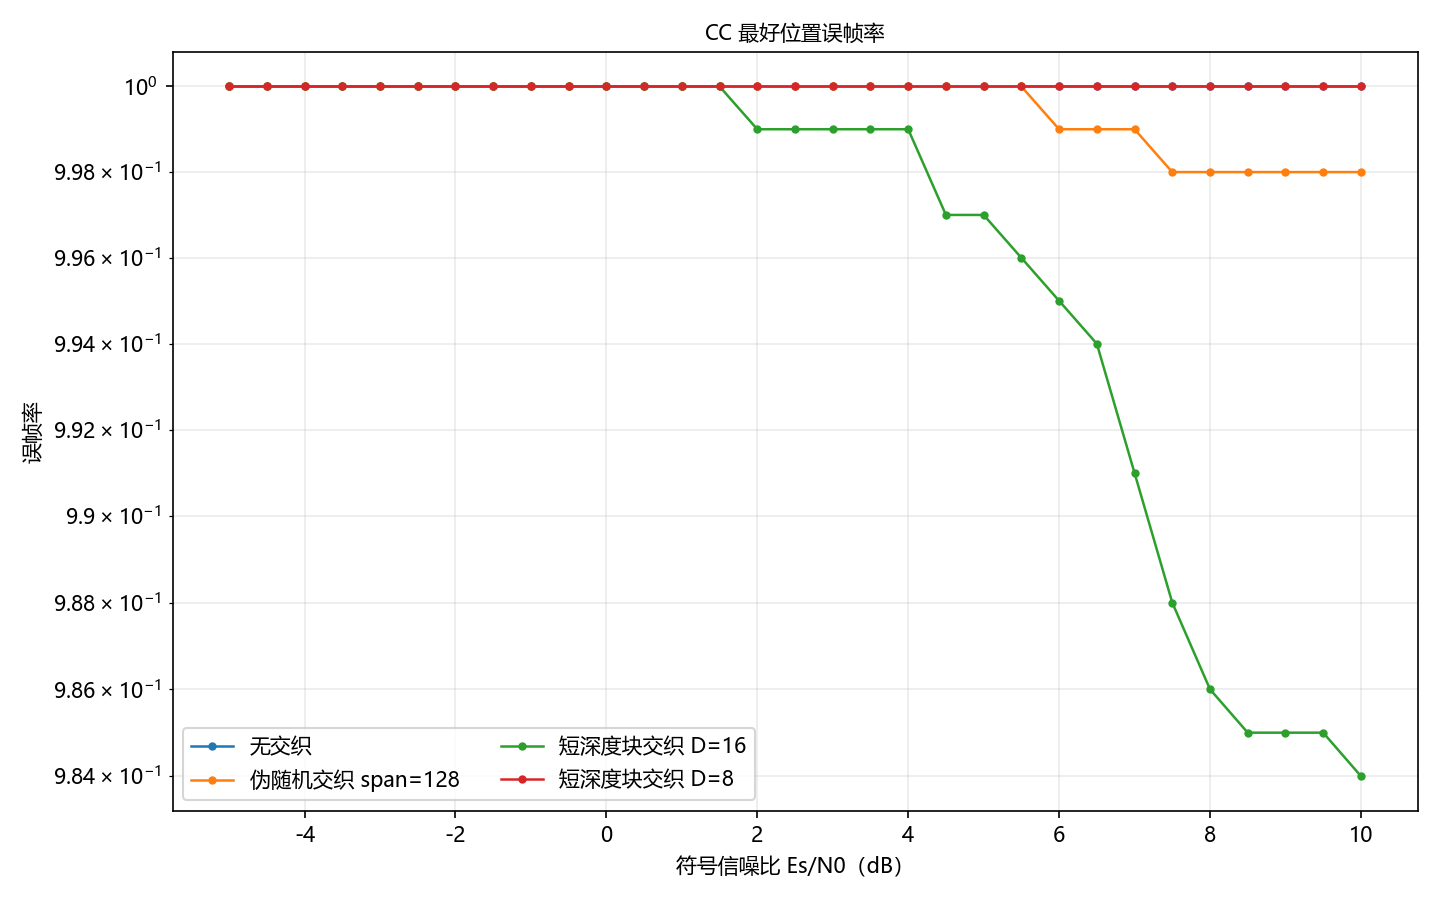
\includegraphics[width=\linewidth]{../Task/Comparison/S7/stage15_scientific_plots/results/cc/09_min_position_fer/figure.png}\\[-0.2em]\small（c）最好位置
  \end{minipage}
  \caption{5\%突发条件下卷积码位置统计结果}
  \label{fig:s7-cc-position-statistics}
\end{figure}

\begin{figure}[htbp]
  \centering
  \begin{minipage}[t]{0.49\textwidth}
    \centering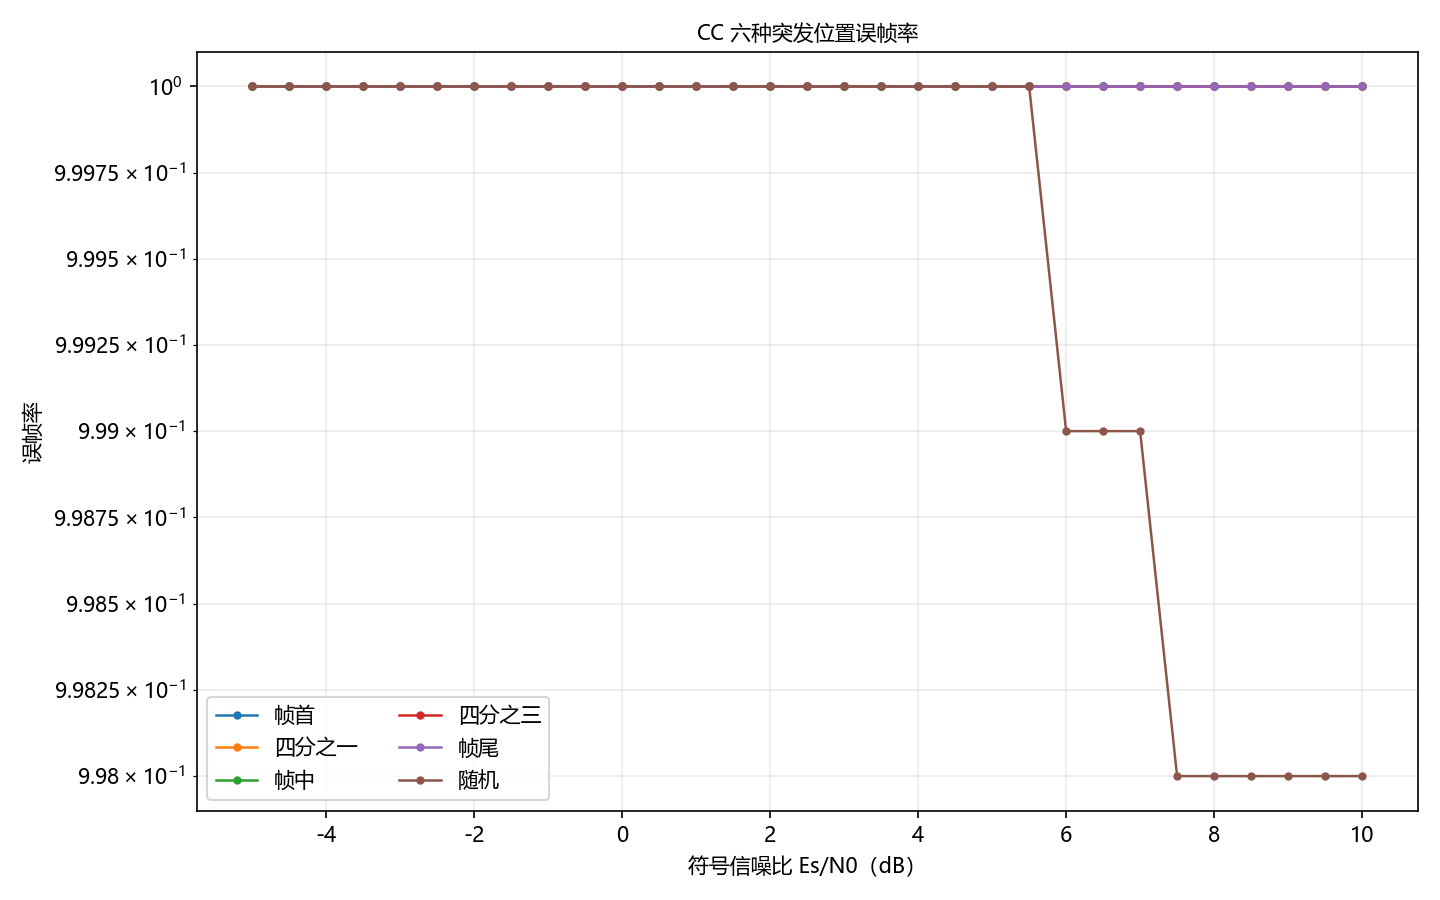
\includegraphics[width=\linewidth]{../Task/Comparison/S7/stage15_scientific_plots/results/cc/06_six_positions_fer/figure.png}\\[-0.2em]\small（a）六位置FER
  \end{minipage}\hfill
  \begin{minipage}[t]{0.49\textwidth}
    \centering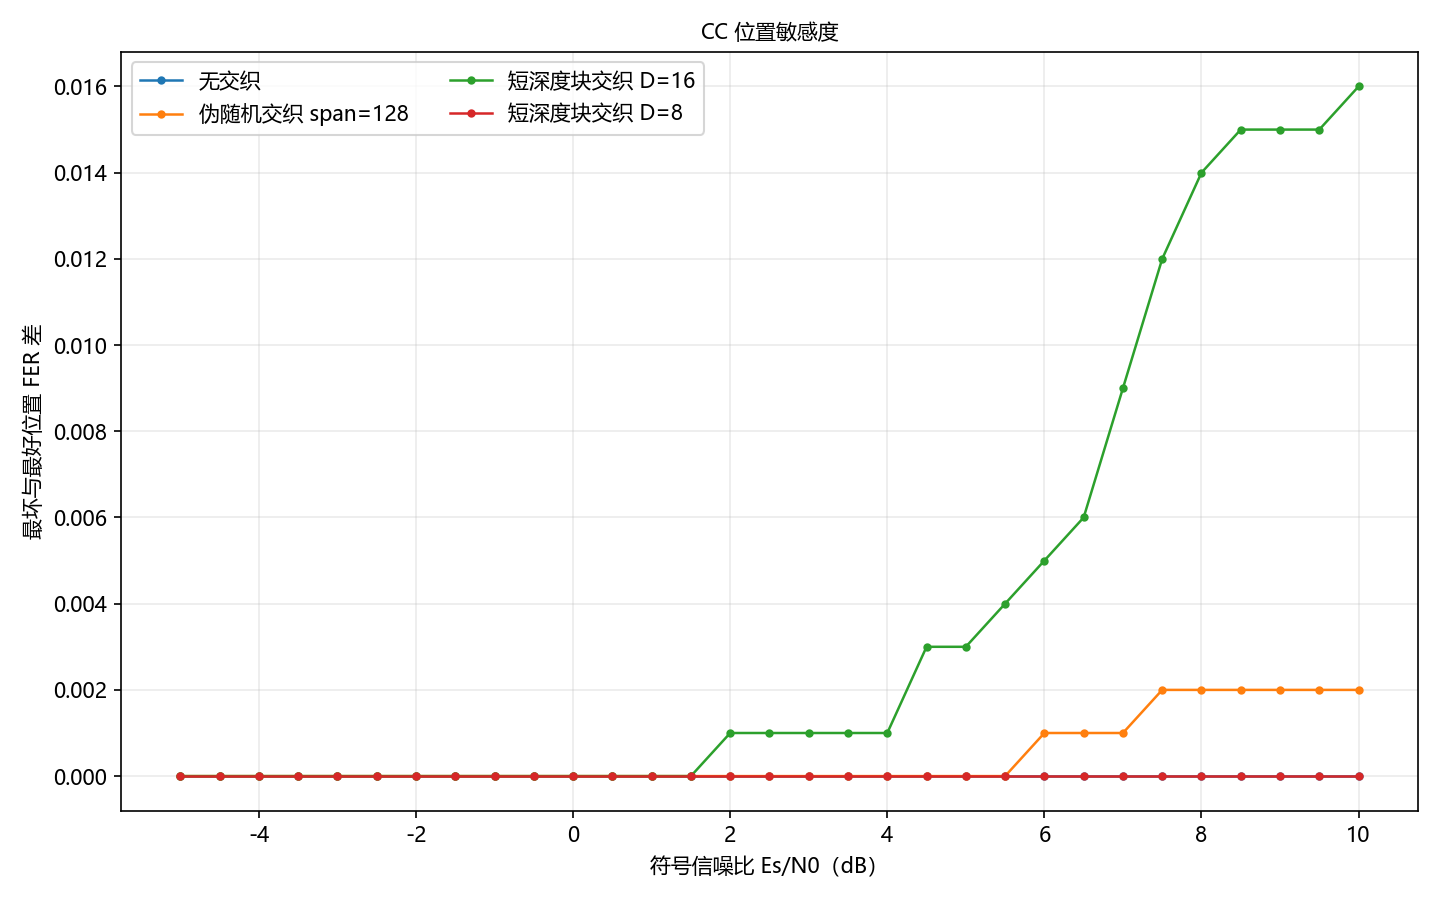
\includegraphics[width=\linewidth]{../Task/Comparison/S7/stage15_scientific_plots/results/cc/10_position_sensitivity/figure.png}\\[-0.2em]\small（b）位置敏感度
  \end{minipage}
  \caption{5\%突发条件下卷积码突发位置敏感性}
  \label{fig:s7-cc-position-detail}
\end{figure}

\subsection{短深度参数与等跨度受控比较}

卷积码的机理不同于BCH子块分散。连续异常集中在相邻trellis step时，会连续改变多个分支度量并影响局部路径竞争；交织把异常观测映射到更远的trellis位置，从而降低连续局部异常同时作用于相邻路径判决的程度。该映射不改变卷积码自由距离，也不改变编码器本身的理论纠错能力。

图\ref{fig:s7-cc-controlled}区分两类问题。左图比较同一规则块交织方法内部的$D=8$与$D=16$，反映深度与跨度变化；右图比较跨度均为128 trellis step、缓存均为256 bit的$D=16$与Pseudo128，反映相同资源边界下排列方式变化。$10$ dB、2\%条件下，$D=16$平均FER为0.718629，Pseudo128为0.448905，当前数据支持伪随机排列在该受控点具有更低FER。5\%条件下两者均接近饱和，差异不支持稳定的低FER排序。

\begin{figure}[htbp]
  \centering
  \begin{minipage}[t]{0.49\textwidth}
    \centering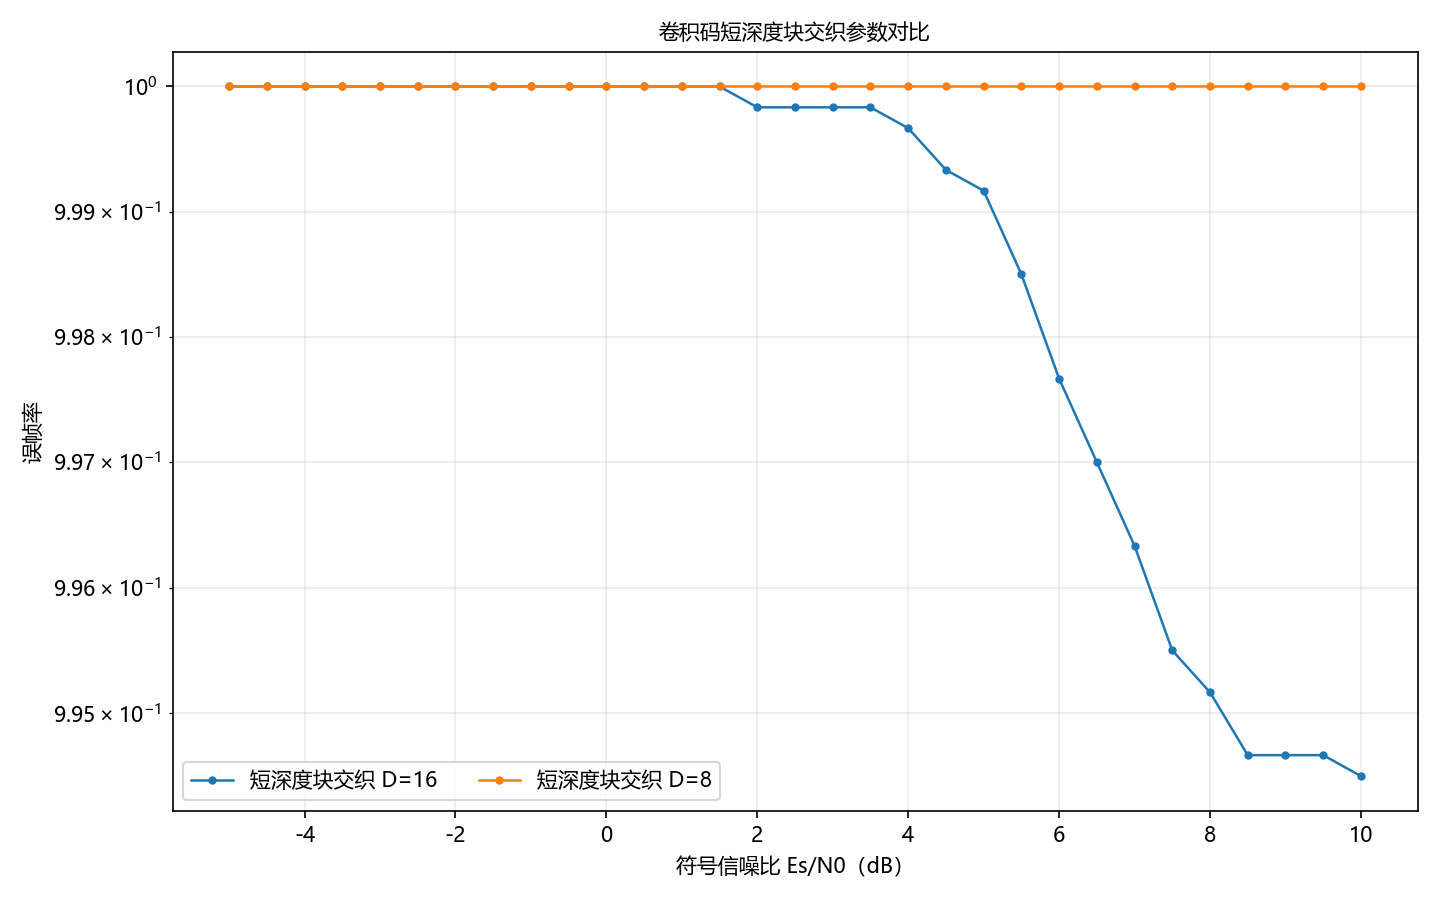
\includegraphics[width=\linewidth]{../Task/Comparison/S7/stage15_scientific_plots/results/cc/14_short_depth_parameters/figure.png}\\[-0.2em]\small（a）短深度参数比较
  \end{minipage}\hfill
  \begin{minipage}[t]{0.49\textwidth}
    \centering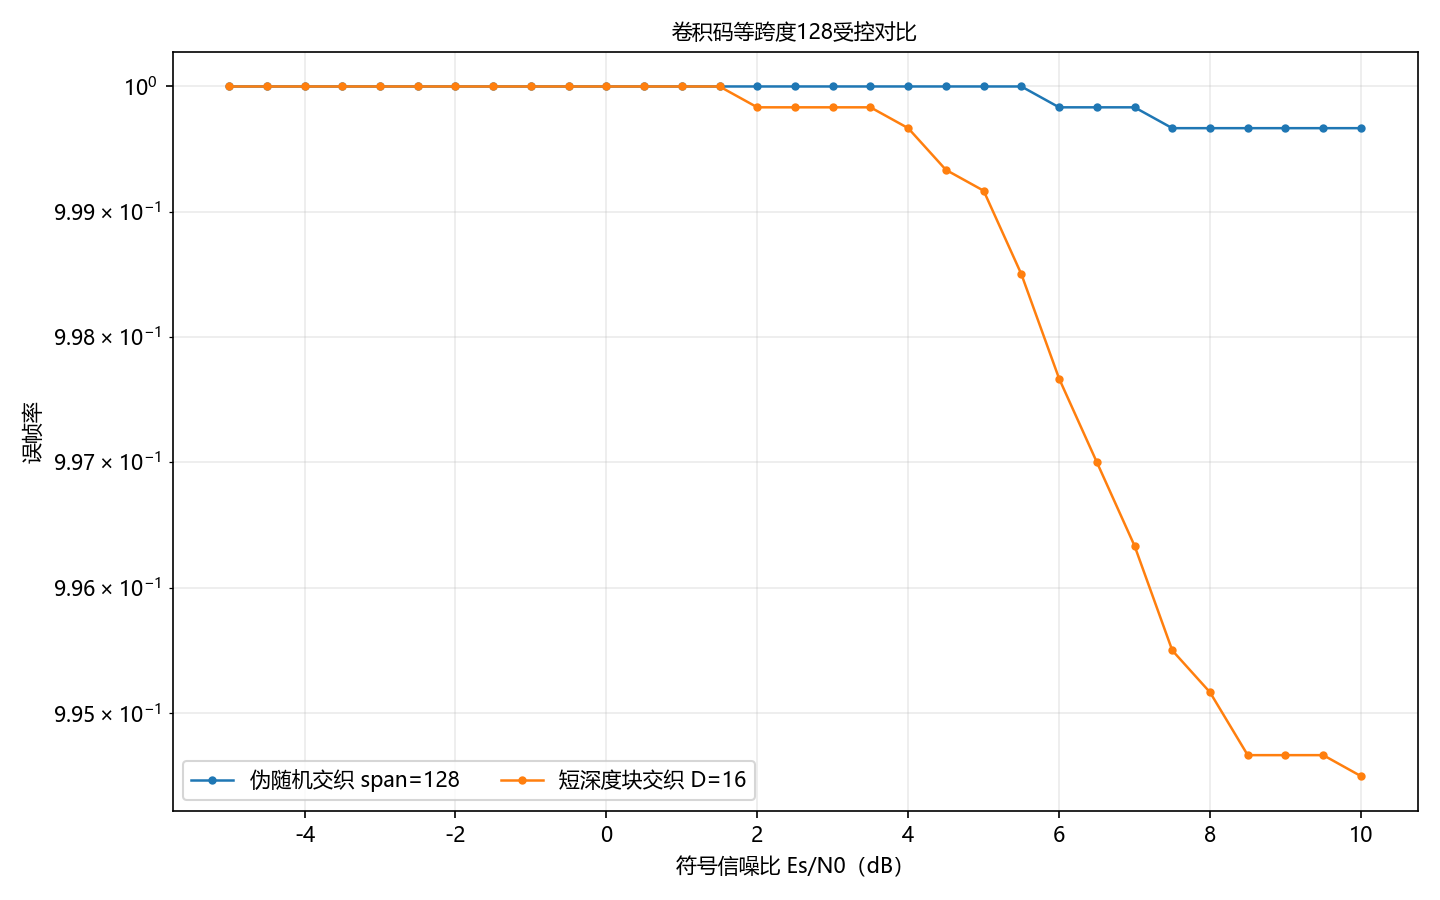
\includegraphics[width=\linewidth]{../Task/Comparison/S7/stage15_scientific_plots/results/cc/15_equal_span_128_controlled/figure.png}\\[-0.2em]\small（b）等跨度128受控比较
  \end{minipage}
  \caption{卷积码短深度与等跨度交织比较}
  \label{fig:s7-cc-controlled}
\end{figure}

\begin{table}[htbp]
  \centering
  \caption{卷积码短深度与等跨度受控比较（$E_s/N_0=10$ dB）}
  \label{tab:s7-cc-controlled}
  \footnotesize
  \begin{tabular}{clrrrp{0.26\textwidth}}
    \toprule
    突发 & 配置 & trellis跨度 & 缓存/bit & 平均FER & 比较角色 \\
    \midrule
    2\% & $D=8$ & 64 & 128 & 0.552654 & 低缓存工程配置 \\
    2\% & $D=16$ & 128 & 256 & 0.718629 & 等跨度规则排列 \\
    2\% & Pseudo128 & 128 & 256 & 0.448905 & 等跨度伪随机排列 \\
    5\% & $D=8$ & 64 & 128 & 1 & 低缓存工程配置 \\
    5\% & $D=16$ & 128 & 256 & 0.994500 & 等跨度规则排列 \\
    5\% & Pseudo128 & 128 & 256 & 0.999667 & 等跨度伪随机排列 \\
    \bottomrule
  \end{tabular}
\end{table}

图\ref{fig:s7-cc-fer-gain}给出5\%条件下的FER改善量。大部分工作点的改善接近零，且局部可能出现负改善，说明增大交织深度并不保证收益持续增加。当前数据中，Pseudo128在2\%高工作点具有较低平均FER；$D=8$以一半缓存获得可观测FER下降；$D=16$虽然增加到相同256 bit缓存，但并未形成一致优于$D=8$或Pseudo128的结果。性能随$D$增大并非单调改善，收益取决于突发长度、位置与排列结构。

\begin{figure}[htbp]
  \centering
  \begin{minipage}[t]{0.49\textwidth}
    \centering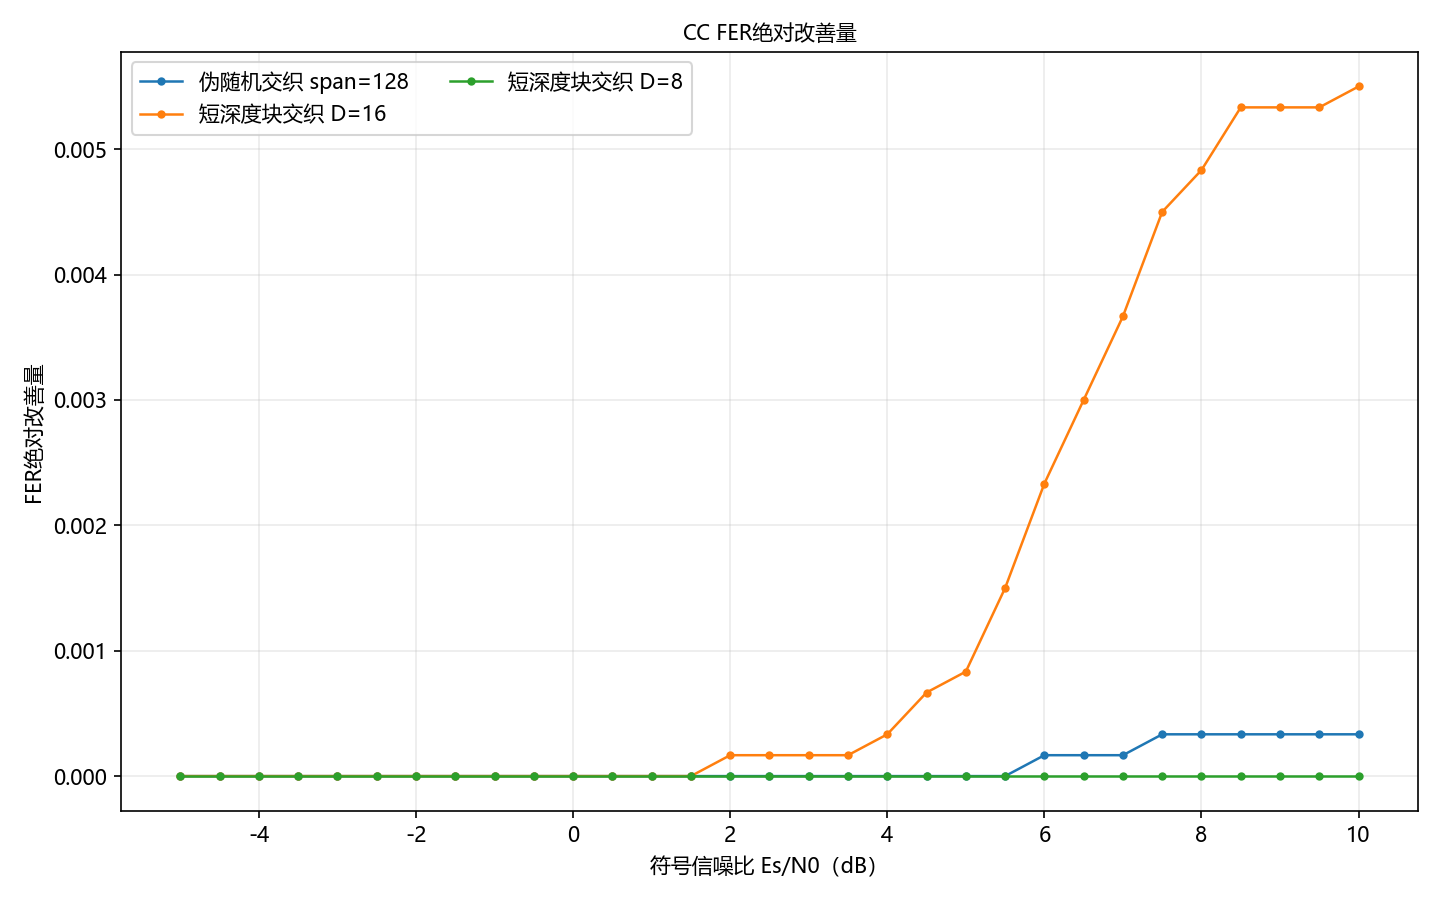
\includegraphics[width=\linewidth]{../Task/Comparison/S7/stage15_scientific_plots/results/cc/11_absoluteFerImprovement/figure.png}\\[-0.2em]\small（a）FER绝对改善量
  \end{minipage}\hfill
  \begin{minipage}[t]{0.49\textwidth}
    \centering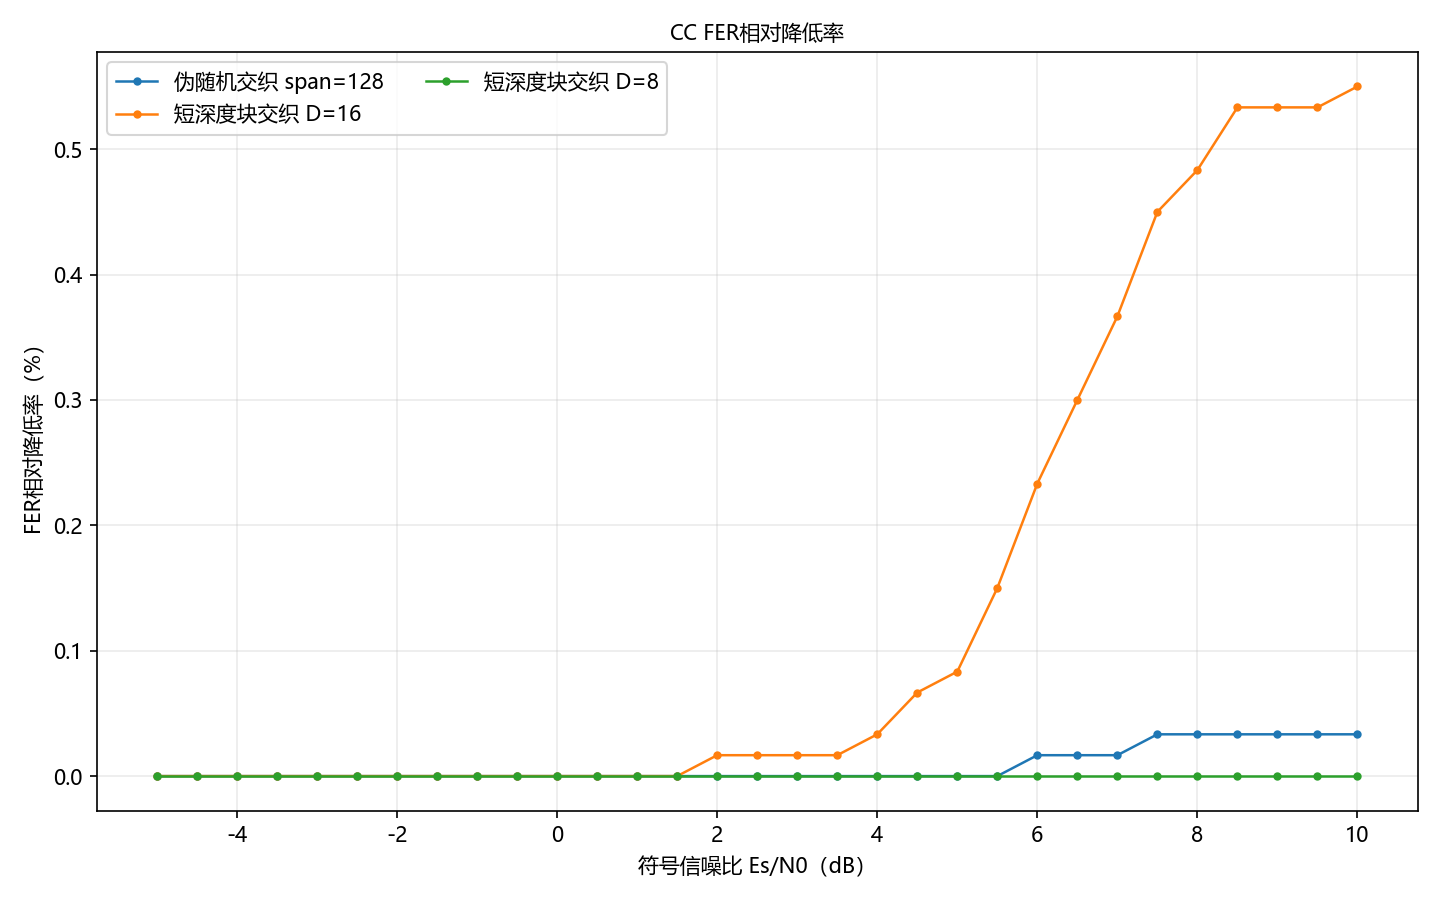
\includegraphics[width=\linewidth]{../Task/Comparison/S7/stage15_scientific_plots/results/cc/12_relativeFerReductionPercent/figure.png}\\[-0.2em]\small（b）FER相对降低率
  \end{minipage}
  \caption{5\%突发条件下卷积码交织的FER改善}
  \label{fig:s7-cc-fer-gain}
\end{figure}

\subsection{FER改善与突发错误容限}

卷积码高工作点容限结果显示，2\%条件下各交织配置的最坏位置FER均高于0.1，5\%条件下则均为1。因此，本章不把任何卷积码配置标记为通过该容限门限。与此同时，六位置平均FER仍能区分2\%条件下的配置差异：Pseudo128最低，$D=8$次之，$D=16$较高。平均性能与最坏位置门限回答的是不同问题，前者衡量总体配置收益，后者约束对突发起点敏感的业务风险。

在配置选择上，$D=8$以128 bit缓存取得44.73\%平均FER下降，Pseudo128以256 bit缓存取得55.11\%下降。增加128 bit缓存对应约10.38个百分点的平均FER相对降低差异，但最坏位置FER只从0.85变为0.84。若业务更重视平均帧成功率，可采用Pseudo128；若缓存受限且允许较高平均FER，$D=8$提供更紧凑的选择。该折中只适用于本章300 bit、终止整帧软Viterbi链路和已测试的2\%突发条件。

\subsection{缓冲需求与软件处理时间}

卷积码缓存量见图\ref{fig:s7-cc-buffer}。$D=8$需要暂存128个编码比特；$D=16$和Pseudo128均需要256个编码比特。按2\%和5\%正式仿真数据重新加权后，三种交织配置的交织CPU时间为737.4、742.7和751.8 ns/帧，去交织CPU时间为384.2、426.9和390.8 ns/帧，译码CPU时间约为$306.6\sim307.5~\mu$s/帧。与无交织配置相比，这些软件函数时间没有形成数量级增长；结构缓存则从0增加至128或256 bit。由于没有统一编码比特率或符号率，本章不把缓存量换算为微秒或毫秒。

\begin{figure}[htbp]
  \centering
  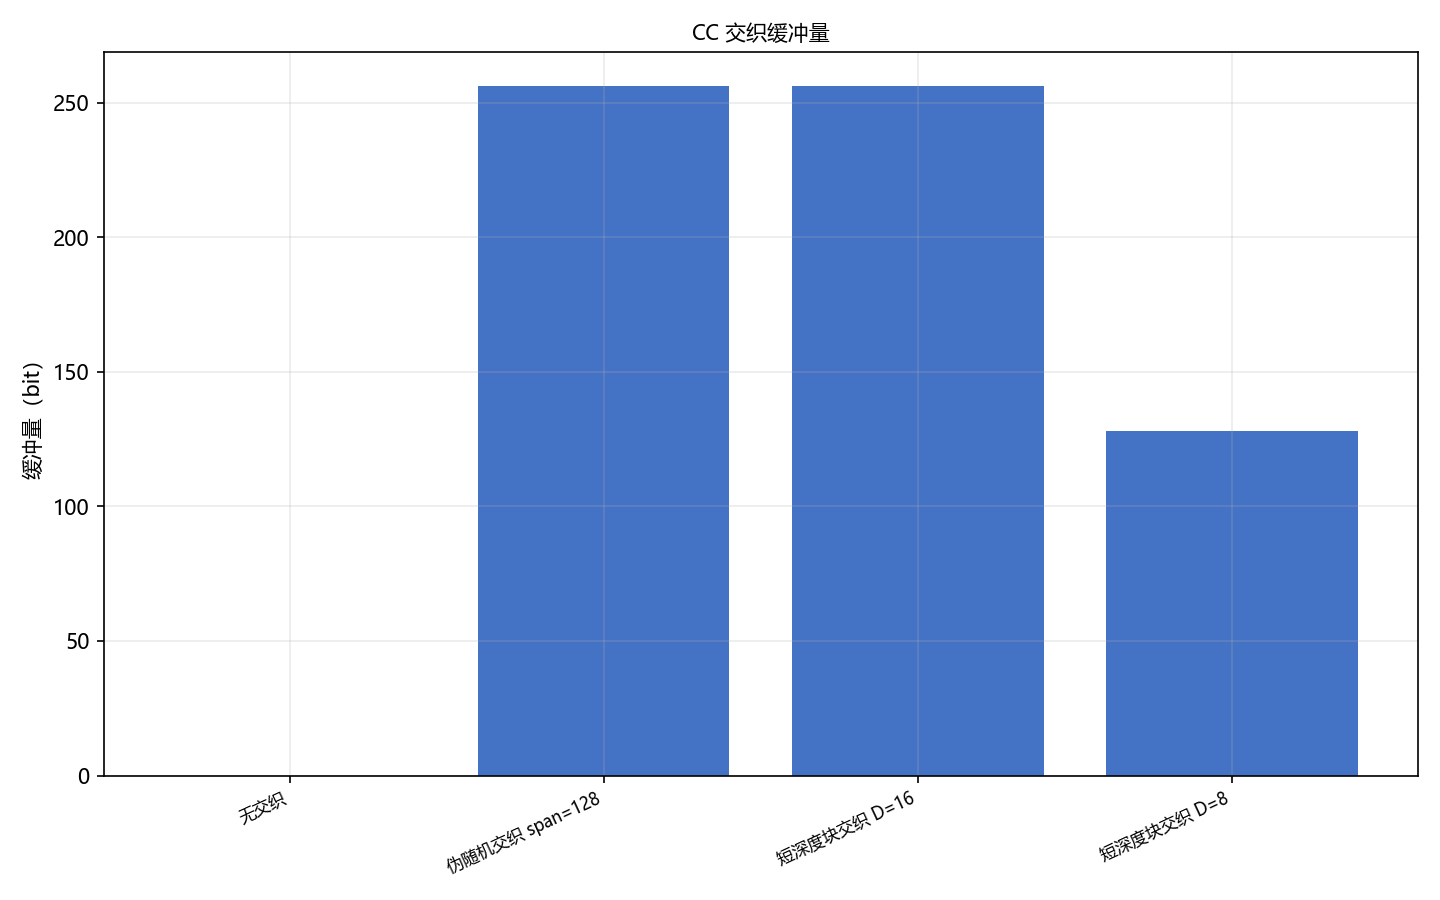
\includegraphics[width=0.88\textwidth]{../Task/Comparison/S7/stage15_scientific_plots/results/cc/19_bufferBits/figure.png}
  \caption{卷积码交织配置的结构缓存量}
  \label{fig:s7-cc-buffer}
\end{figure}

\section{LDPC无交织近码率基线}

本节只比较无突发AWGN条件下的卷积码与LDPC N640基线。两者有效载荷均为300 bit，实际码率分别为0.490196和0.468750，相对码率差约4.375\%。LDPC采用BG2、$Z=40$、layered NMS译码，归一化系数0.80，最多32次迭代；两种方案均不使用交织。表\ref{tab:s7-cc-ldpc-baseline}中的BER和FER取$E_s/N_0=0.5$ dB正式点，软件译码时间为各自正式AWGN点的帧数加权参考。

\begin{table}[htbp]
  \centering
  \caption{卷积码与LDPC无交织近码率基线}
  \label{tab:s7-cc-ldpc-baseline}
  \footnotesize
  \resizebox{\textwidth}{!}{%
  \begin{tabular}{lrrrrrlp{4.2cm}}
    \toprule
    方案 & 载荷/bit & 发送/bit & 码率 & FER & BER & 译码CPU/ns每帧 & 角色 \\
    \midrule
    卷积码 & 300 & 612 & 0.490196 & 0.0048944 & $7.29\times10^{-5}$ & 428650 & 无交织、无突发AWGN参考 \\
    LDPC N640 & 300 & 640 & 0.468750 & $6.0\times10^{-5}$ & $1.0\times10^{-6}$ & 93743 & 无交织、无突发AWGN近码率参考 \\
    \bottomrule
  \end{tabular}}
\end{table}

图\ref{fig:s7-cc-ldpc-latency}给出相同加权口径的软件译码CPU时间参考。卷积码可描述306个trellis step、64状态及分支度量与加比选过程；LDPC可描述N640、边消息更新和平均迭代，但两类操作不能直接相加为统一操作数，也不能把该软件时间直接解释为硬件实现时延。

\begin{figure}[htbp]
  \centering
  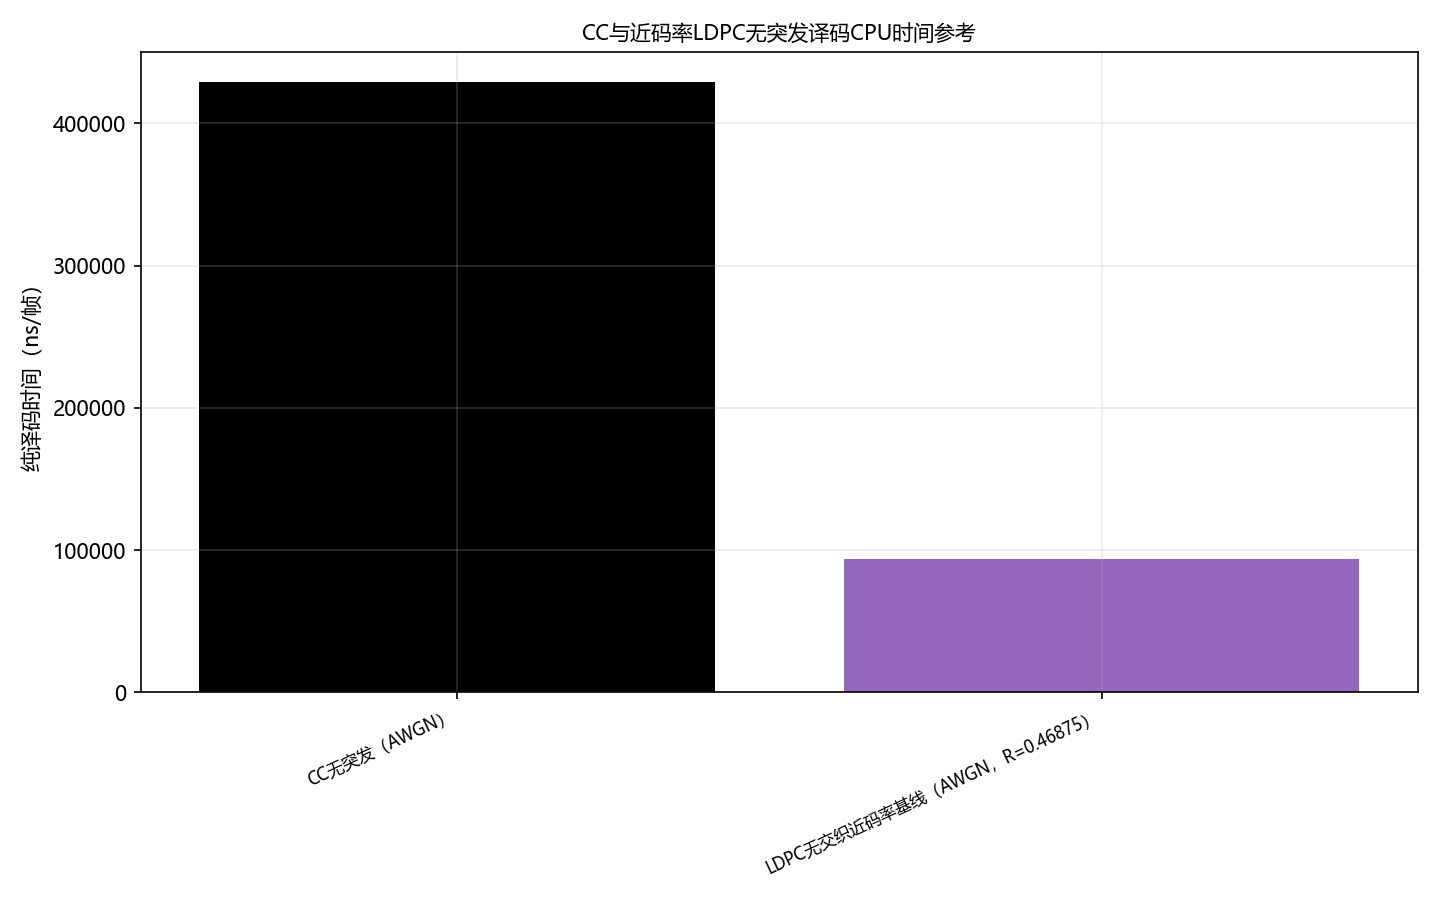
\includegraphics[width=0.88\textwidth]{../Task/Comparison/S7/stage15_scientific_plots/results/cc/22_cc_ldpc_no_burst_decode_latency/figure.png}
  \caption{卷积码与LDPC无交织、无突发AWGN软件译码CPU时间参考}
  \label{fig:s7-cc-ldpc-latency}
\end{figure}

该基线能够说明：在接近码率和相同有效载荷下，当前LDPC实现的AWGN误码、误帧结果及软件译码时间可作为高速编码方案参照。它不能说明LDPC在2\%或5\%突发条件下的性能，也不能给出LDPC的交织收益、突发容限或位置敏感性。LDPC不进入本章交织配置排名。

\section{交织收益与工程代价综合分析}

表\ref{tab:s7-buffer-time}统一列出仅按2\%和5\%正式仿真数据加权的软件时间。BCH三种交织方法均缓存285 bit，交织与去交织函数合计约$0.65~\mu$s/帧；卷积码$D=8$缓存128 bit，Pseudo128和$D=16$缓存256 bit，交织与去交织函数合计约$1.12\sim1.17~\mu$s/帧。软件CPU时间不等价于物理链路等待，缓存bit数也不等价于时延数值。工程实现仍需结合实际编码比特率、存储结构和硬件并行度换算。

\begin{table}[htbp]
  \centering
  \caption{交织缓存与软件CPU处理时间（仅2\%和5\%行加权）}
  \label{tab:s7-buffer-time}
  \footnotesize
  \begin{tabular}{llrrrr}
    \toprule
    方案 & 配置 & 缓存/bit & 交织/ns & 去交织/ns & 译码/ns \\
    \midrule
    BCH & 无交织 & 0 & 328.4 & 310.5 & 8424 \\
    BCH & 子块结构$D=19$ & 285 & 324.9 & 329.9 & 8998 \\
    BCH & 行列$R=15$ & 285 & 325.3 & 322.6 & 8886 \\
    BCH & 全帧伪随机 & 285 & 325.1 & 324.6 & 8755 \\
    卷积码 & 无交织 & 0 & 745.8 & 404.4 & 307767 \\
    卷积码 & 短深度$D=8$ & 128 & 737.4 & 384.2 & 307483 \\
    卷积码 & Pseudo128 & 256 & 751.8 & 390.8 & 307488 \\
    卷积码 & 短深度$D=16$ & 256 & 742.7 & 426.9 & 306640 \\
    \bottomrule
  \end{tabular}
\end{table}

高工作点最坏位置FER见表\ref{tab:s7-burst-tolerance}。在当前测试网格与FER不高于0.1的判据下，BCH子块结构和行列交织均通过2\%与5\%条件；无交织和全帧伪随机配置未通过。卷积码四种配置在2\%和5\%的最坏位置均未通过该门限。该表只描述已测试的两档条件，不在网格之间插值，也不把LDPC加入突发错误容限判断。

\begin{table}[htbp]
  \centering
  \caption{高工作点突发错误容限（最坏位置FER）}
  \label{tab:s7-burst-tolerance}
  \footnotesize
  \begin{tabular}{llrrrr}
    \toprule
    方案 & 配置 & 2\%长度/bit & 2\%最坏FER & 5\%长度/bit & 5\%最坏FER \\
    \midrule
    BCH & 无交织 & 6 & 1 & 14 & 1 \\
    BCH & 子块结构$D=19$ & 6 & $4.40\times10^{-4}$ & 14 & 0.00102 \\
    BCH & 行列$R=15$ & 6 & $5.00\times10^{-4}$ & 14 & $8.80\times10^{-4}$ \\
    BCH & 全帧伪随机 & 6 & 0.99998 & 14 & 1 \\
    卷积码 & 无交织 & 12 & 1 & 31 & 1 \\
    卷积码 & 短深度$D=8$ & 12 & 0.85 & 31 & 1 \\
    卷积码 & Pseudo128 & 12 & 0.84 & 31 & 1 \\
    卷积码 & 短深度$D=16$ & 12 & 1 & 31 & 1 \\
    \bottomrule
  \end{tabular}
\end{table}

综合建议见表\ref{tab:s7-engineering-recommendation}。对本章200 bit分块BCH方案，行列$R=15$在两档突发高工作点均取得最低六位置平均FER，可作为性能优先配置；子块结构$D=19$的结果接近，并具有与19个BCH子块直接对应的结构解释。两者缓存相同，软件处理时间差异很小。全帧伪随机置换虽覆盖相同跨度，但位置稳定性和平均FER均不足以替代两种规则结构方案。

对300 bit卷积码，配置选择需要区分性能与缓存目标。Pseudo128在2\%高工作点获得最低平均FER，但需要256 bit缓存；$D=8$以128 bit缓存获得44.73\%的平均FER下降，可作为缓存优先配置。$D=16$增加到256 bit缓存后未形成稳定增益，说明单纯增加深度的收益趋于不稳定。5\%条件下各配置FER接近饱和，因此当前证据不支持将任何卷积码交织配置描述为31 bit突发下的低FER方案。

\begin{table}[htbp]
  \centering
  \caption{S7工程配置建议}
  \label{tab:s7-engineering-recommendation}
  \small
  \begin{tabular}{p{0.13\textwidth}p{0.25\textwidth}p{0.18\textwidth}p{0.34\textwidth}}
    \toprule
    方案 & 建议配置 & 适用目标 & 证据边界 \\
    \midrule
    分块BCH & 行列$R=15$ & 性能优先 & 两档高工作点平均FER最低；仅限本章200 bit分块方案 \\
    分块BCH & 子块结构$D=19$ & 结构清晰备选 & 性能接近行列方案；不改变单块理论纠错能力 \\
    卷积码 & 短深度$D=8$ & 缓存优先 & 128 bit缓存；与Pseudo128不是等跨度纯方法比较 \\
    卷积码 & Pseudo128 & 2\%条件FER优先 & 256 bit缓存；5\%条件下未形成低FER工作点 \\
    \bottomrule
  \end{tabular}
\end{table}

\section{本章结论}
\enlargethispage{5\baselineskip}

本章在固定编码与译码方案下比较了2\%和5\%连续突发错误。对200 bit分块BCH方案，无交织时错误集中在较少的15 bit子块，单块多错误事件频繁；子块结构交织和行列交织把异常分散到约14个子块，并在$10$ dB、5\%条件下把单块最大错误数从15降至2，使更多子块落入BCH(15,11,1)原有单比特可纠正范围。两种规则结构交织的平均FER均由无交织的1降至$10^{-3}$以下，其中行列$R=15$为$7.63\times10^{-4}$。该结论限定于本章采用的分块BCH方案。

对300 bit卷积码，连续异常集中作用于相邻trellis step并改变局部路径度量竞争；交织将异常观测映射到更远的trellis位置。2\%条件下，$10$ dB处$D=8$和Pseudo128的平均FER分别为0.552654和0.448905，均低于无交织的1；5\%条件下所有配置仍接近FER饱和。$D=8$与Pseudo128是不同跨度和缓存规模的工程配置，$D=16$与Pseudo128才构成128 trellis step等跨度受控比较。增大$D$没有形成单调收益，交织也没有改变卷积码自由距离。

工程代价方面，BCH规则结构交织需要285 bit缓存，卷积码$D=8$与Pseudo128分别需要128 bit和256 bit缓存。仅按正式展示条件加权的软件交织与去交织时间均远小于对应译码函数时间，但这些CPU测量不能替代物理链路时延。LDPC N640只提供无交织、无突发AWGN近码率参考，能够支持高速编码方案的AWGN性能与软件实现对照，不能支持突发错误性能、交织排名或位置敏感性结论。
